



%Autor: Nico Schrodt, Andreas Schmider
%September 2021 - Mai 2022


\documentclass[12pt]{article}

\usepackage{multicol}
\usepackage{geometry}
\usepackage{blindtext}
\usepackage{setspace}
\usepackage{hyperref}
\usepackage[headsepline=0.8pt, footsepline =0.8pt]{scrlayer-scrpage}
\usepackage{listings}
\usepackage{subcaption}
\usepackage{tabularx}
\usepackage{xurl} %Formats \url{}-entrys better
\usepackage{color, colortbl}
\usepackage{pdfpages}
\usepackage{amssymb}
\usepackage{float}

\geometry{a4paper, top=25mm, left=35mm, right=25mm, bottom=25mm, headsep=13mm, footskip=12mm, head=14.5pt}

\lstset{mathescape=true,
        literate=
               {->}{$\rightarrow{}$}{1},
        }

%encoding
%--------------------------------------
\usepackage[utf8]{inputenc}
\usepackage[T1]{fontenc}
%--------------------------------------

%German-specific commands
%--------------------------------------
\usepackage[ngerman]{babel}
%--------------------------------------

%Hyphenation rules
%--------------------------------------
\usepackage{hyphenat}
%--------------------------------------

\usepackage{graphicx}
\usepackage{subcaption}
\graphicspath{ bilder/}


\newcommand{\Autor}{Andreas Schmider, Nico Schrodt}

\newcommand{\Bearbeitungszeitraum}{2 Semester}
\newcommand{\Kurs}{TINF19B3}
\newcommand{\Betreuer}{Prof. Dr.-Ing. Kai Becher}

\newcommand{\DHBWLogoDeckblatt}{
\includegraphics[width=4.5cm]{Logos/dhbw-logo}}
\newcommand{\IntelDataLines}{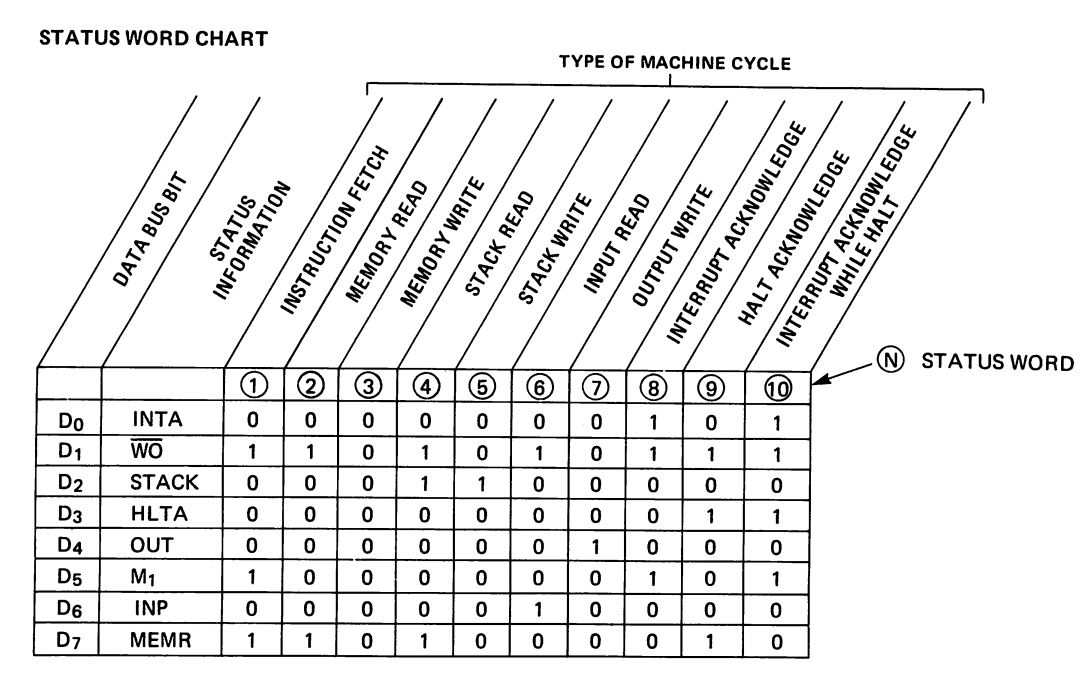
\includegraphics[width=15cm]{Bilder/Intel8080_DataLines}}

\newcommand{\Titel}{Konzeptionierung eines Simulators für einen 8-Bit Prozessor}
\newcommand{\ArtArbeit}{Studienarbeit}
\newcommand{\Abschluss}{Bachelor of Science}
\newcommand{\Studiengang}{Studiengang Informationstechnik}

\newcommand{\Ort}{Karlsruhe}


\newcommand{\imgSpaceBefore}{\vspace{10pt}}
\newcommand{\todo}{\textbf{TODO}}


\newcounter{applabelno}
\newcommand{\applabel}[1]{\refstepcounter{applabelno}\label{#1}}
\renewcommand{\theapplabelno}{\Alph{applabelno}}


%\newcommand{\Abgabedatum}{16.02.2021}


\begin{document}
\onehalfspacing
\pagenumbering{Roman}
	\begin{titlepage}
		{\DHBWLogoDeckblatt}\\[2cm]
		\begin{center}
			\vspace*{-2cm}
			{\Huge \Titel}\\[2cm]
			{\Huge \ArtArbeit}\\[2cm]
			{\Large \Abschluss}\\[0.5cm]
			{\large \Studiengang}\\[0.5cm]
			{\large an der}\\[0.5cm]
			{\large Dualen Hochschule Baden-Württemberg Karlsruhe}\\[0.5cm]
			{\large von}\\[0.5cm]
			{\large\bfseries \Autor}\\[1cm]
			{\large Abgabedatum \today}
			\vfill
		\end{center}
		\begin{tabular}{l@{\hspace{1cm}}l}
			Bearbeitungszeitraum & \Bearbeitungszeitraum \\
			Kurs & \Kurs \\
%			Ausbildungsfirma & \Ausbildungsfirma \\
			Betreuer & \Betreuer \\
		\end{tabular}
	\end{titlepage}

\newpage

\thispagestyle{empty}
\begin{center}
\Large\bfseries Erklärung
\end{center}
\medskip
\noindent
Wir versichern hiermit, dass wir unsere \ArtArbeit \ mit
dem Thema: 
\begin{center}
	 \Titel \ 
\end{center}
selbstständig verfasst und keine anderen als die angegebenen Quellen und
Hilfsmittel benutzt haben. Wir versichern zudem, dass die eingereichte elektronische Fassung mit der
gedruckten Fassung übereinstimmt.

\vspace{3cm}
\noindent
\underline{\Ort, \today \hspace{9cm}}\\
%\hfill\underline{\hspace{6cm}}\\
Ort, Datum\hfill Unterschrift\hspace{4cm}

\newpage

\thispagestyle{empty}
\tableofcontents

\newpage

%\thispagestyle{empty}
\thispagestyle{plain}
\cleardoublepage
\addcontentsline{toc}{section}{\listfigurename}
\listoffigures

\addcontentsline{toc}{section}{\listtablename}
\listoftables

\newpage

%\thispagestyle{empty}
\thispagestyle{plain}
\cleardoublepage
\section*{Abkürzungsverzeichnis}
\addcontentsline{toc}{section}{Abkürzungsverzeichnis}
\textbf{ALU} - Arithmetic Logic Unit\\
\textbf{CISC} - Complex Instruction Set Computer\\
\textbf{GUI} - Graphical User Interface\\
\textbf{MISD} - Multiple-instruction stream single-data stream\\
\textbf{MIMD} - Multiple-instruction stream multiple-data stream\\
\textbf{RISC} - Reduced Instruction Set Computer\\
\textbf{SISD} - Single-instruction stream single-data stream\\
\textbf{SIMD} - Single-instruction stream multiple-data stream

\newpage
\pagenumbering{arabic}

%% Kopf und Fusszeilen==================================================== 
\pagestyle{scrheadings} % Seite mit Headern 

% loescht voreingestellte Stile 
\clearpairofpagestyles
%\clearscrheadings 
\clearmainofpairofpagestyles
%\clearscrplain 

% %%% Kopfzeile 
% einseitig: Bei einseitigem Layout, nur folgende Zeilen verwenden !!! 
%\ohead[] {
\includegraphics[height=0.5cm]{Logos/Firmenlogokopfzeile}}
\ihead[]{\leftmark} % links: Kapitel
%\chead[]{} % mitte: 

% %%% Fusszeile 
%\cfoot[]{} % mitte: 
\cfoot[\pagemark]{\pagemark} % rechts: Seitenzahl


% Angezeigte Abschnitte im Header 
\automark{section}  % Inhalt von [\rightmark]{\leftmark} 

\section{Einführung}
Dieses Kapitel befasst sich vorwiegend mit relevanten Grundlagen der Arbeit. Unter anderem wird das Ziel spezifiziert, elementare Aspekte der Arbeitsweise eines Prozessors werden erläutert und die verschiedenen Werkzeuge, mit denen das Ziel realisiert wird, werden aufgeführt.

\subsection{Ziel der Arbeit}
In dieser Arbeit soll ein Simulationsprogramm geschrieben werden, mit dem mehrere unterschiedliche 8-Bit Prozessoren simuliert werden können. Dazu sollen die grundlegenden Eigenschaften in kurzen Lernprogrammen erläutert werden. Ebenfalls soll es eine interaktive Einweisung geben wie der Simulator verwendet werden kann.

\subsection{Repository}
Der Quellcode kann in folgendem GitHub-Repository abgerufen werden:\\ \url{https://github.com/NicoSchrodt/8-Bit-Simulator}

\newpage

\subsection{Theoretische Grundlagen}
Von Nico\\

\noindent
Als Vorbereitung für die Implementierung der verschiedenen Prozessoren werden einige allgemeingültige Architekturprinzipien eines Prozessors erläutert. 

\subsubsection{Architektur eines Prozessors}
Der fundamentale Aufbau eines Prozessors lässt sich in folgende Bausteine einteilen:\\ \\
\textbf{Rechenwerk}\\
Das Rechenwerk ist die zentrale Einheit, mit der eingehende Befehle verarbeitet werden. Es erhält Werte aus dem Speicher und führt damit in der Arithmetisch-logische Einheit (ALU) Operationen durch. Zum Rechenwerk dazugehörig sind auch Hilfsregister, die beispielsweise als naher Zwischenspeicher fungieren.\\ \\
\textbf{Steuerwerk}\\
Das Steuerwerk ist für die korrekte Abarbeitung von Befehlen zuständig. Es besteht aus dem Befehlsdekoder, dem Befehlszähler und einem Statusregister.\\ \\
\textbf{Programmspeicher}\\
Der Programmspeicher eines Prozessors enthält die einzelnen Befehle, welche vom Befehlsdekoder dekodiert werden. Dabei wird der Befehl verwendet, der an der vom Befehlszähler spezifizierten Stelle im Speicher steht.\\ \\
\textbf{Ein-/Ausgabewerk}\\
Das Ein-/Ausgabewerk ist für die Kommunikation des Prozessors mit anderen Systemkomponenten verantwortlich.\\
\subsubsection{Befehlsformate}
Für einen Prozessor wird zwischen vier verschiedenen Befehlsformaten unterschieden. Diese beziehen sich auf die Anzahl der Adressen, welche der ALU bei Beginn einer Operation zur Verfügung gestellt werden. \cite{Adressformate}\\ \\
\textbf{Null-Adress-Anweisungen}\\
Vom Akkumulator (Stack) wird der Wert der zwei obersten Adressfeldern entnommen und die Operation wird auf diese ausgeführt. Der Speicherort des Ergebnisses ist ebenfalls vorbestimmt. Daher werden zum Ausführen von Operationen keine Adressen benötigt.\\ \\
\textbf{Ein-Adress-Anweisungen}\\
Wie bei einer Null-Adress-Anweisung wird ein Wert aus dem Akkumulator entnommen. Ein zweiter Wert wird aus dem Speicher der übergebenen Adresse entnommen. Der Speicherort des Ergebnisses ist nach wie vor fest.\\ \\
\textbf{Zwei-Adress-Anweisungen}\\
Für Zwei-Adress-Anweisungen ist es möglich eine Bezugsadresse für die Operanden anzugeben sowie eine Zieladresse, in der das Ergebnis der Operation gespeichert wird.\\ \\
\textbf{Drei-Adress-Anweisungen}\\
Drei-Adress-Anweisungen sind essentiell komplexere Zwei-Adress-Anweisungen. Eine der drei verfügbaren Adressen wird ebenfalls für die Zieladresse der Operation verwendet. Für das Beziehen der Operanden steht eine weitere Adresse zur Verfügung.\\

\subsubsection{Harvard- und von-Neumann-Architektur}
Von Andreas\\

\noindent
Prozessoren können auf viele unterschiedliche Arten kategorisiert werden. In diesem Kapitel geht es um die Harvard- und von-Neumann-Architektur. 
Für beide Architekturen werden die im vorherigen Kapitel beschriebenen Bauteile benötigt. 
Bei der von-Neumann-Architektur gibt es nur einen Daten-, Steuer- und Adressbus, der mit allem verbunden ist. 
Bei einem neuen Befehl muss somit zuerst ein Befehl vom Speicher in das Steuerwerk geladen werden. 
Erst danach wird mit Steuersignalen den einzelnen Komponenten mitgeteilt was als nächstes geschehen soll. Häufig müssen daraufhin Daten geladen oder geschrieben werden. 
Damit der Speicher aber weiß woher die Daten gelesen werden müssen, muss zuerst die Adresse über den Bus geschickt werden. 
Dadurch, dass es bei der von-Neumann-Architektur nur einen Bus gibt, muss darüber die ganze Kommunikation ablaufen.
\\
Die Harvard-Architektur besitzt mehrere, getrennte Busse, da es auch zwei getrennte Speicher gibt: 
Einen Programmspeicher und einen Datenspeicher. 
Bei der von-Neumann-Architektur gibt es nur einen Speicher.
Deshalb müssen Programmcode und Daten zwangsweise zusammen abgelegt werden. 
Dadurch, dass bei der Harvard-Architektur zwei getrennte Speicher verwendet werden und jeder einen eigenen Bus besitzt, können sich Befehle und Daten nicht gegenseitig blockieren. 
Somit können beide Speicher parallel angesprochen und verwendet werden. 
Während für den vorherigen Befehl noch Daten eingelesen werden, kann schon ein neuer Befehl aus dem Programmspeicher eingelesen werden. 
Daraus ergibt sich, rein aus der Theorie schon, eine höhere Ausführungsgeschwindigkeit als bei von-Neumann-Systemen. 
Der Nachteil davon ist allerdings, dass Bauteile öfters verwendet werden, was dazu führt, dass diese Prozessoren teurer sind.
Deshalb sind heutzutage auch die meisten Prozessoren noch mit einer von-Neumann-Architektur. \cite{Architektur_stud}, \cite{Architektur}

\subsubsection{CISC und RISC}
Von Andreas\\

\noindent
Ein Prozessor unterstützt immer nur eine gewisse Menge an Befehlen, dies wird Instruction Set genannt. Heutzutage gibt es zwei grundlegende Prozessorarchitekturen: Complex Instruction Set Computer (CISC) und Reduced Instruction Set Computer (RISC). Früher konnten Prozessoren genau einer dieser Gruppen zugeordnet werden, allerdings ist das bei den heutigen Prozessoren nicht mehr möglich, da sowohl RISC- als auch CISC-Befehle dem Prozessor zur Verfügung gestellt werden, um die Vorteile von beiden zu nutzen.
\\\\
Bei CISC-Prozessoren wird versucht, soviel Arbeit wie möglich in einem Befehl ausführen zu können. So gibt es viele verschieden Befehle, die auch unterschiedlich viel Zeit benötigen. Dadurch wird es aber auch möglich, komplexere Befehle direkt in der Hardware zu berechnen. Bei diesen Befehlen gibt es auch einige Adressierungsarten mehr als bei RISC-Prozessoren. Für vorbestimmte Aufgaben gibt es auch eigene Register, die nur dafür verwendet werden, und davon auch nur wenige. Ein Nachteil der CISC-Prozessoren ist, dass die eigenen Befehle erst noch durch ein Mikroprogramm interpretiert werden müssen und dieses die komplexen Befehle in mehrere kleine Befehle aufteilen muss, welche erst dann vom Prozessor bearbeitet werden können. Dies kostet etwas mehr Zeit und verlangsamt die Ausführung. Die Mikroprogramme, die dafür verwendet werden, werden in einem kleinen Read-only Memory (ROM) gespeichert.
\\\\
Bei RISC-Prozessoren wird versucht mit nur wenigen, kleinen Befehlen auszukommen. Diese sind wiederum sehr schnell, da sie meist fest verdrahtet sind, müssen aber mit anderen kombiniert werden um die Komplexität eines einzigen CISC-Befehls zu erreichen.  Im Gegensatz zu CISC-Prozessoren besitzen RISC-Prozessoren viele Register, die frei verwendbar sind und nicht für spezielle Operationen bestimmt sind. Ebenso können die meisten Befehle in nur einem einzigen Arbeitsschritt ausgeführt werden.  \cite{Herold}
\\\\
Da bei CISC-Prozessoren mit nur einem Befehl viel berechnet werden kann, sind diese optimal für Übersetzer oder Interpreter geeignet. Bei der Entwicklung können einzelne komplexe Befehle anstatt vieler kleiner verwendet werden. Jedoch können RISC-Prozessoren schneller Befehle ausführen, da:

\begin{itemize}
\item es nur wenige Befehle gibt und diese schnell dekodiert werden können.
\item die Befehle mithilfe von Pipelines effizienter abgearbeitet werden können.
\item kein Mikroprogramm die einzelnen Befehle erst noch interpretieren muss.
\end{itemize}


\subsubsection{Parallelität nach Flynn}
Von Andreas\\

Von Michael Flynn wurden 1966 die folgenden vier Arten von Parallelisierung eingeführt: \cite{Flynn}

\begin{itemize}
\item Single-instruction stream, single-data stream (SISD)
\item Single-instruction stream, multiple-data stream (SIMD)
\item Multiple-instruction stream, single-data stream (MISD)
\item Multiple-instruction stream, multiple-data stream (MIMD)
\end{itemize}

\noindent
\textbf{SISD}\\
Diese Beschreibung trifft auf die einfachen Einprozessorsysteme zu. Dabei kann immer nur eine Operation gleichzeitig ausgeführt werden und diese werden in nur einer möglichen Reihenfolge aus einem Datenstrom abgearbeitet.\\

\noindent
\textbf{SIMD}\\
Bei SIMD werden Pipelines eingesetzt, die es ermöglichen, mehrere korrekte Abfolgen von Programmbefehlen auszuführen. So können unterschiedliche Programme in sich selbst in der richtigen Reihenfolge, aber mit anderen Programmen abwechselnd ausgeführt werden.\\

\noindent
\textbf{MISD}\\
Diese Variante scheint auf Anhieb keinen effizienten Nutzen zu besitzen, da mehrere Prozessoren alle die gleichen Befehle ausführen, die aus einem Daten-Strom stammen. Dies kann aber dazu verwendet werden, die Korrektheit durch Redundanzen zu bestätigen. \\

\noindent
\textbf{MIMD}\\
Diese Architektur verwendet mehrere Prozessoren und mehrere Daten-Ströme. Heutzutage ist dies unter dem Begriff Mehrprozessorsysteme bekannt. So werden für jeden einzelnen Prozessor ein Datenstrom erzeugt, der unabhängig von den anderen Prozessoren arbeiten kann. Dabei ist es für die Prozessoren aber trotzdem möglich, die Daten der anderen Prozessoren zu nutzen. Nur durch MIMD oder MISD, also die Ausführung mit mehreren unabhängigen Prozessoren, ist es möglich, Programme tatsächlich parallel ablaufen zu lassen. Mit SISD oder SIMD sind nur quasi-parallele Ausführungen möglich.\\

\newpage

\section{Projektplanung und Verlauf}
Von Andreas\\

\noindent
Bei Projektbeginn wurde kein konkretes Ziel vorgegeben. Es wurde nur verlangt, dass ein Simulator für 8-Bit Prozessoren entwickelt werden soll. Deshalb wurde zu Beginn die Entscheidung getroffen, dass eine kleine Lernsoftware entwickelt werden soll. Der Simulator sollte ursprünglich fähig sein, mehrere unterschiedliche Prozessoren simulieren zu können. Damit sollten die Unterschiede verschiedener Prozessoren dargestellt und dem Anwender vermittelt werden. Jedoch hat sich bei der Untersuchung von mehreren Prozessoren herausgestellt, dass es nur geringe Unterschiede zwischen den Prozessoren gibt. Zwar hat jeder Prozessor seine Eigenheiten, die aber für den Anwender kaum bemerkbar sind. Der größte Unterschied sind die verschiedenen Befehlssätze. Die meisten Prozessoren verwenden für die gleichen Befehle unterschiedliche Mnemonics und Bitkombinationen. Sobald aber die Befehle dekodiert wurden, läuft im Prozessor meistens sehr Ähnliches oder sogar Gleiches ab. Dabei kann es vorkommen, dass ein Prozessor noch ein zusätzliches Register z.B. als Zwischenspeicher verwendet, welches die anderen nicht besitzen. Aber wie die Daten im Prozessor hin- und her geschoben werden und die Befehle, die die ALU ausführt, unterscheidet sich zwischen den Prozessoren kaum oder ist sogar identisch. Deshalb wurde sich später dafür entschieden, dass nicht mehrere, sondern nur ein Prozessor simuliert werden soll.
\\\\
Bei dem Multi-Prozessor-Simulator war geplant, dass nur die Befehle direkt ausführbar sein sollen. Sodass eine assemblierte Quellcode-Datei eingelesen und ausgeführt werden kann. Diese Implementierung hat sichergestellt, dass die zwangsweise notwendigen Eigenschaften simuliert werden. Dazu zählt, dass die Inhalte von Registern, die vom Anwender verwendet werden können, nach der Ausführung der Befehlen die korrekten Werte enthalten. Zusätzlich dazu wurden auch die Flags simuliert, da diese für den korrekten Programmablauf notwendig sind.
\\\\
Der Single-Prozessor-Simulator sollte etwas genauer darstellen, wie ein Prozessor arbeitet. Dafür wurde der Intel 8080 als Prozessor ausgewählt. Ein Intel 8080-Befehl besteht aus mindestens einem und maximal fünf bzw. in diesem Simulator sechs Maschinenzyklen. Jeder dieser Maschinenzyklen wiederum aus drei bis fünf Zuständen. Ein kompletter Befehl besteht, bei dem Intel 8080, insgesamt aus mindestens 4 und maximal 18 Zuständen. Mit dieser Implementierung kann jeder einzelne Zustand nachvollzogen werden. Dadurch werden auch die W- und Z-Register verwendet, auf die der Anwender normalerweise keinen Zugriff hat und deshalb beim Multi-Prozessor-Simulator nicht beachtet wurden.
\\

\noindent
Die Aufgabengebiete bei diesem Simulator waren klar verteilt. Nico Schrodt hat sich um das Frontend, also die graphische Oberfläche, und Andreas Schmider um das Backend, also die Funktionsweise des Prozessors gekümmert. Diese zwei Bereiche können gut voneinander getrennt werden. Somit musste sich nur auf wenige Schnittstellen geeinigt werden.


\newpage

\subsection{Multi-Prozessor-Simulator}
Mit diesem Simulator soll es möglich sein, mehrere unterschiedliche Prozessoren simulieren zu können. Vor der Implementierung des Simulators müssen ein oder mehrere geeignete Prozessoren ausgewählt werden. In den nachfolgenden Kapiteln werden einige potenzielle Kandidaten näher analysiert und beschrieben.

\subsubsection{Z80}
\todo
Fällt vermutlich weg

\subsubsection{Intel 8080}
Da der Intel 8080 in dem Single-Prozessor-Simulator verwendet wird und dort auch detaillierter implementiert wird, wird dieser auch dort in Kapitel \ref{SPS} beschrieben.


\newpage

\subsection{Single-Prozessor-Simulator}
\label{SPS} 
Von Andreas\\ 

\noindent
Als Prozessor für den Single-Prozessor-Simulator wurde der Intel 8080 ausgewählt. Der Intel 8080 bietet ein breites Spektrum an Befehlen und ist repräsentativ für einen der ersten großen, kommerziell erfolgreichen Prozessoren.

\subsubsection{Register}
\label{RegisterSection}

Der Intel 8080 besitzt ein SRAM-Array mit 16-Bit-Registern. Darin enthalten sind der Programmzähler mit 16 Bit und der Stack Pointer mit 16-Bit. Dazu gibt es noch acht weitere 8-Bit Register. Diese können entweder alleine oder zusammen mit einem anderen 8-Bit Register als ein 16-Bit Register verwendet werden. Dabei gibt es aber nur die fest vorgegebenen Kombinationen. Das B- und C-Register, das D- und E-Register, das H- und L- Register und die temporären W- und Z- Register. Die W- und Z-Register können nicht vom Programmierer verwendet werden und dienen nur zur internen Ausführung von Befehlen. Bei manchen Befehlen wird der Stackpointer als 16-Bit Register verwendet.
Über einen Multiplexer ist es möglich, 8 Bit auf den internen Adressbus zu schreiben oder von dort zu lesen. Über das Adress-Latch des Inkrementer/Dekrementer-Chipsatzes ist es möglich 16 Bit aus den Registern an den Adress-Puffer weiterzuleiten. \cite{IntMan16}


\imgSpaceBefore
\begin{figure}[h]
\centering
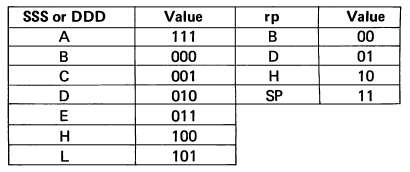
\includegraphics[width=10cm]{Bilder/register_kodierung}
\caption{Kodierung der Register \cite{IntMan30}}
\label{fig:register_kodierung}
\end{figure}

\subsubsection{Befehle}

Der Intel 8080 ist in der Lage, aus einem, zwei oder drei Bytes bestehen Befehle auszuführen. Dabei gibt das erste Byte immer den Operation Code an. In Byte zwei und drei werden nur Daten oder Adressen gespeichert. Dabei werden die zwei Byte großen Adressen so gespeichert, dass das niederwertige Byte vor dem höherwertigem gespeichert wird. Die Adressen können dabei über vier verschiedene Modi verwendet werden.

\begin{itemize}
\item Direct
\item Register
\item Register Indirect
\item Immediate
\end{itemize}

\noindent
Bei \glqq Direct\grqq\ wird der Wert im Speicher mit der angegebenen Adresse verwendet. Hier werden das Low-Byte im zweiten und das High-Byte im dritten Byte gespeichert. Bei \glqq Register\grqq\ wird auf ein oder zwei Register verwiesen und der Register-Typ verhält sich wie bei \glqq Direct\grqq. Bei \glqq Register Indirect\grqq\ wird der Wert aus der Adresse aus dem zweiten und dritten Byte des Befehls gelesen. Dieser Wert wird als Adresse verarbeitet und erst der Wert aus dieser Adresse ist der zu verwendende Wert. Bei \glqq Immediate\grqq\ steht
im zweiten und/oder dritten Byte ein Wert, mit dem gearbeitet wird (Low-Byte im zweiten Byte).
Bei Interrupts und Verzweigungs-Befehlen gibt es nur die \glqq Direct\grqq - und \glqq Register indirect\grqq -Modi. \cite{IntMan45}
\\ 

\noindent
Der Prozessor besitzt fünf Condition-Flags. Das Zero-Flag gibt an ob das Ergebnis eines Befehls den Wert 0 hatte. Das Sign-Flag gibt an, ob Bit 8, das Most Signifikant-Bit, des letzten Ergebnisses den Wert 1 hat. Wenn das letzte Ergebnis gerade war, ist das Paritäts-Flag gesetzt. Das Carry-Flag zeigt an ob es einen Übertrag bei einer Addition oder einen Abzug bei einer Subtraktion oder einem Vergleich gab. Das Auxiliary Carry-Flag zeigt ebenfalls einen Übertrag oder Abzug an, aber zwischen Bit 3 und Bit Bit 4. \cite{IntMan45}
\\

\subsubsection{OP-Code Kodierung}
\label{chapter:opcode}
Jedem Befehl ist ein Byte (OP-Code) zugewiesen. Dabei gibt es mehrere Typen. In manchen Befehlen werden einzelne Bits verwendet, um Register oder Registerpaare zu kodieren, während in anderen jedes Bit verwendet wird. In Tabelle \ref{table:opcode} sind die verschiedenen Möglichkeiten aufgelistet. Bei dem Befehl ACI ist es wichtig, dass das Byte genau 0xC7 ist. Bei ADC und INR wird ein 8-Bit Register in den Befehl kodiert. Hierbei wird unterschieden, ob Daten in das Register geschrieben (DDD für Destination) oder daraus gelesen (SSS für Source) werden. Bei Mov r1, r2 wird sowohl aus einem Register gelesen als auch in ein anderes geschrieben, weshalb nur noch zwei Bit für den eigentlichen MOV-Befehl übrig bleiben. Bei dem INX-Befehl wird ein 16-Bit Register verwendet. Wie auf Seite \pageref{RegisterSection} beschrieben, können auch zwei 8-Bit-Register zu einem 16-Bit-Register zusammen geschlossen und damit verwendet werden. Insgesamt gibt es davon drei Kombinationen. Dementsprechend werden in diesen Befehlen diese Register mit zwei Bit kodiert. Damit gibt es noch eine weitere Bitkombination, mit der ein weiteres Register verwendet werden kann. Mit der vierten noch übrig gebliebenen Kombination wird der Stackpointer als 16-Bit-Register verwendet.

\begin{table}[h]
\centering
\begin{tabular}{|l|c|c|c| } 
 \hline
 Befehl & OP-Code \\
 \hline 
 ACI & \texttt{1100 1110} \\ 
 ADC r & \texttt{1000 1SSS} \\
 INR r & \texttt{00DD D101} \\
 MOV r1, r2 & \texttt{01DD DSSS} \\
 INX rp & \texttt{00RP 0011} \\
 \hline
\end{tabular}
\caption{OP-Code-Typen \cite{IntMan30}}
\label{table:opcode}
\end{table}

\subsubsection{Befehlsgruppen}
Jeder Befehl kann genau einer der folgenden fünf Gruppen zugeordnet werden. Jede Gruppe verhält sich anders mit den Status-Flags. So gibt es eine Gruppe, bei der die meisten Befehle alle Flags ändern, aber auch Gruppen, wobei die meisten Befehle kein einziges Flag verändern.
\\

\noindent
\textbf{Daten-Transfer-Gruppe}\\
Für den Prozessor sind 13 Befehle aus dieser Gruppe bekannt. Bei keinem dieser Befehle werden die Condition Flags gesetzt oder zurückgesetzt. Alle Befehle, die dieser Gruppe angehören, schreiben ausschließlich Daten in Register oder in den Programmspeicher. Es werden keine Rechenoperationen oder Sprünge ausgeführt. Zu dieser Gruppe gehören die folgenden Befehle:

\begin{multicols}{2}
\begin{itemize}
\item Move Register
\item Move from Memory
\item Move to Memory
\item Move immediate
\item Move to Memory Immediate
\item Load register pair immediate
\item Load Accumulator direct
\item Store Accumulator direct
\item Load H and L direct
\item Store H and L direct
\item Load Acumulator indirect
\item Store Accumulator indirect
\item Exchange H and L with D and E
\end{itemize}
\end{multicols}

\vspace{10pt}
\noindent
\textbf{Arithmetikgruppe}\\
Dieser Gruppe gehören 20 Befehle an. Die meisten dieser Befehle beeinflussen alle Statusflags. Ausnahmen bilden dabei der INR- und DCR-Befehl, der INX- und DCX-Befehl und der DAD-Befehl. Der INR- und DCR-Befehl beeinflussen alle Flags außer das Carry-Flag. Der DAD-Befehl verändert ausschließlich das Carry-Flag. Keine Flags werden bei dem INX- und DCX-Befehl beeinflusst. Zu dieser Gruppe gehören die Befehle, die arithmetische Operation ausführen, also z.B. Additionen oder Subtraktionen.


\begin{multicols}{2}
\begin{itemize}
\item Add Register
\item Add Memory
\item Add immediate
\item Add Register with carry
\item Add Memory with carry
\item Add immediate with carry
\item Sustract Register
\item Subtract Memory
\item Subtract immediate
\item Subtract Register with borrow
\item Subtract Memory with borrow
\item Subtract immediate with borrow
\item Increment Register
\item Increment Memory
\item Decrement Register
\item Decrement Memory
\item Increment register pair
\item Decrement register pair
\item Add register pair to H and L
\item Decimal Adjust Accumulator
\end{itemize}
\end{multicols}

\vspace{10pt}
\noindent
\textbf{Logische Gruppe}\\
Aus dieser Gruppe sind 19 Befehle bekannt. Diese Gruppe enthält Befehle, die logische Operationen wie UND und ODER ausführen. Bis auf die Rotations-, die Komplement- und den Set-Carry-Befehl werden immer alle Flags beeinflusst.

\begin{multicols}{2}
\begin{itemize}
\item AND Register
\item AND Memory
\item AND immediate
\item Exclusive OR Register
\item Exclusive OR Memory
\item Exclusive OR immediate
\item OR Register
\item OR Memory
\item OR immediate
\item Compare Register
\item Compare Memory
\item Compare immediate
\item Rotate left
\item Rotate right
\item Rotate left through Carry
\item Rotate right through Carry
\item Complement Accumulator
\item Complement Carry
\item Set Carry
\end{itemize}
\end{multicols}

\vspace{10pt}
\noindent
\textbf{Verzweigungsgruppe}\\
Zu dieser Gruppe werden die Befehle dazu gezählt, die den standardmäßigen Programmablauf verändern. Keiner dieser Befehle verändert ein Flag. Der Intel 8080 kennt eigentlich nur einen Conditional-Befehl pro Sprung/Call etc. Für den Assembler können aber eigene Mnemonics für die unterschiedlichen Flags verwendet werde.

\begin{itemize}
\item Jump
\item Conditional Jump
\item Call
\item Conditional Call
\item Return
\item Conditional Return
\item Restart
\item Jump H and L indirect - move H and L to PC
\end{itemize}

\vspace{10pt}
\noindent
\textbf{Stapel-, Ein/Ausgangs-, und Maschinenkontrollgruppe}\\
Die Befehle, die dieser Gruppe angehören, verändern entweder den Stack, interne Status-Flags oder sind für Ein- und Ausgaben zuständig. Zusätzlich dazu wird auch der NOP-Befehl (No Operation) dazu gezählt, obwohl er keines der Kriterien erfüllt. Letztendlich kann der NOP-Befehl keiner Gruppe genau zugewiesen werden, da dieser keine Funktion besitzt.
In dieser Gruppe verändert nur der POP-Befehl die Flags.

\begin{multicols}{2}
\begin{itemize}
\item Push
\item Push Processor status word
\item Pop
\item Pop processor status word
\item Exchange stack top with H and L
\item Move HL to SP
\item Input
\item Output
\item Enable Interrupts
\item Disable Interrupts
\item Halt
\item No op
\end{itemize}
\end{multicols}


\subsubsection{Typen der Maschinenzyklen}
Jeder Befehl oder Befehlszyklus benötigt mindestens einen und maximal fünf Maschinenzyklen zum kompletten Ausführen des Befehls. Dabei kann jeder Maschinenzyklus genau einem Typ zugeordnet werden. Die existierenden Befehlstypen sind:

\begin{itemize}
\item Fetch
\item Memory Read
\item Memory Write
\item Stack Read
\item Stack Write
\item Input
\item Output
\item Interrupt
\item Halt
\item Halt Interrupt
\end{itemize}

\noindent
Der erste Maschinenzyklus ist immer ein Fetch-Zyklus. Bei diesem wird immer ein neuer Befehl eingelesen und dekodiert. Für alle anderen Maschinenzyklenphasen kann nicht mehr genau gesagt werden zu welchem Typ diese gehören. Deshalb wird in dem ersten Zustand jedes Maschinenzyklus immer der Befehlstyp während des SYNC-Taktes auf den Datenbus kodiert. \cite{IntMan18}


\subsubsection{Interrupts}
Der Intel 8080 ist in der Lage Interrupts auszuführen, die den normalen Programmfluss unterbrechen. Dies ist aber nur zwischen Befehlen möglich. Wenn ein Interrupt eintritt, während ein Befehl noch ausgeführt wird, wird dieser zuerst bis zum Schluss noch ausgeführt. Eine Besonderheit der Interrupts ist, dass jeder Interrupt ein Byte mitliefert, das angibt, was der Interrupt ausführen soll. Dabei ist jeder Befehl erlaubt, der nur ein Byte benötigt. Somit kann auch nur ein Befehl ausgeführt werden. Damit aber auch größere Interrupt Service Routines möglich sind gibt es den RST-Befehl. Dieser Befehl schreibt, den aktuellen Programmzähler auf den Stack und springt an eine von acht Stellen im Programmspeicher. Welche Stelle genau wird im RST-Befehl dekodiert. Diese acht Sprungpunkte liegen alle genau acht Byte auseinander. Falls dies aber für den Interrupt nicht ausreicht, kann von dort an eine andere Stelle im Programmspeicher gesprungen werden. Da der Intel 8080 eine von-Neumann-Architektur verwendet und der Stack an einer beliebigen Stelle im Programmspeicher (64kB) liegen kann, gibt es so gut wie keine Größenlimitierung dafür. Bei manchen anderen Prozessoren kann der Stack z.B. maximal acht Einträge besitzen. Für den Intel 8080 wurde es ermöglicht, dass Interrupts durch andere Interrupts unterbrochen werden können. Durch den RST-Befehl wird der momentane Programmzähler immer auf den Stack geschrieben. Somit kann immer der neueste Interrupt ausgeführt werden und kann dann zum zuvor ausgelösten Interrupt zurückspringen.


\newpage

\section{Umsetzung}
Von Nico\\

\noindent
In diesem Kapitel wird darauf eingegangen, wie die in Kapitel 2 erarbeitete Analyse der ausgewählten Prozessoren implementiert wird.

\subsection{Abstraktion der Architektur}
Der Prozessor wird in verschiedene Unterklassen aufgeteilt. Dabei ist vorgesehen, dass dies in einer Art Sternstruktur aufgebaut wird, das heißt die verschiedenen Bestandteile des Prozessors sollen alle mit einer zentralen Klasse interagieren, aber nicht untereinander.

\subsubsection{Prozessor}
Die Prozessor-Klasse soll die zentrale Einheit des Simulators sein. Über diese sollen sowohl Anfragen über Informationen vorgenommen werden, zum Beispiel um diese in der Benutzeroberfläche anzuzeigen, als auch Instruktionen an den Prozessor als ganzes gesendet werden. Dabei ist zwischen zwei Arten von Anfragen zu unterscheiden, gültigen und ungültigen. Gemeint sind damit Anfragen die in einem echten Prozessor zulässig wären, beispielsweise einen externen Bus zu befüllen oder die nächste Anweisung auszuführen, und Anfragen, die unzulässig wären, wie den Programmzähler manuell zu setzen.

\subsubsection{ALU}
Die ALU soll die Bearbeitung logischer Operationen im Prozessor simulieren, um ein möglichst genaues Bild jedes Zustandes des Prozessors darzustellen, statt beispielsweise solche Operationen manuell in der Prozessor-Klasse abzuarbeiten. Im Verlauf des Projektes wrude die Entscheidung getroffen, das Ausführen der verschiedenen Operationen eher zu emulieren als zu simulieren. Um eine entsprechende Genauigkeit zu gewährleisten, werden deshalb nicht ganze Instruktionen, sondern die einzelnen Maschinenzyklen und Zustände ausgeführt.

\subsubsection{Register}
Die Register-Klasse soll ähnlich wie die ALU den Zugriff auf Register möglichst realitätsgetreu simulieren. Dabei sollen Methoden, die den Zugriff regeln, ähnlich aufgebaut werden wie es im echten Prozessor möglich wäre.

\subsubsection{Peripherie}
Mit der Peripherie soll alles abgedeckt werden, was nicht Teil der zentralen Bestandteile ist, also der Register oder der ALU. Dazu zählt zum Beispiel ein externer Datenbus oder Schnittstellen für Taktsignal o.Ä.

\subsection{Möglichkeiten der Simulation}
Um einen Ablauf für die Simulation festzulegen, muss zuerst bestimmt werden, welche Parameter eingestellt, welche Optionen verändert, und welche Operationen im Simulator durchgeführt werden können. Geplant ist, dass die Simulation zu jedem Zeitpunkt unterbrechbar sein soll. Der kleinste Zeitabschnitt, für den dies sinnvoll ist, wäre ein einzelner Zustand eines Maschinenzyklus. Es ist geplant, dass alle in der Register-Klasse modellierten Register auch in der Benutzeroberfläche dargestellt und manipuliert werden können. Zu manipulierbaren Registern soll auch der Programmspeicher zählen. Dieser soll entweder manuell oder über eine externe Datei befüllbar sein. Für das externe Befüllen muss der für den Simulator vorgegebene Assembler \cite{Assembler} verwendet werden. Die Manipulation des Speichers soll auch während der Simulation möglich sein.

\subsection{Aufbau der GUI}
\label{chp:AufbauGUI}
Das Simulieren des Prozessors ist die ein Aspekt des Projekts. Gleichermaßen wichtig für einen funktionierenden Simulator ist aber auch die Benutzeroberfläche, mit der dieser bedient wird. In diesem Abschnitt werden die einzelnen Aspekte dieser analysiert.
\subsubsection{Hauptmenü}
Bei Programmstart wird das in Abbildung \ref{fig:Hauptmenue} gezeigte Fenster mit dem Hauptmenü geöffnet.\imgSpaceBefore

\begin{figure}[H]
\centering
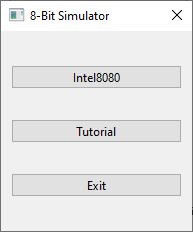
\includegraphics[width=6cm]{bilder/Hauptmenue}
\caption{Hauptmenü}
\label{fig:Hauptmenue}
\end{figure}

\noindent
Die Aufgabe dieses Fensters ist simpel. Es gibt drei verschiedene Knöpfe, die jeweils eine Funktion erfüllen:
\begin{itemize}
	\item Intel8080: Öffnet das Simulationsfenster des Intel 8080-Prozessors
	\item Tutorial: Öffnet ein Fenster mit einer kurzen Einweisung in die Handhabung des Simulators für den Intel 8080
	\item Exit: Schließt das Fenster und alle laufenden Hintergrundprozesse, für den Fall, dass ein Simulatorprozess in der selben Session verwendet wurde.
\end{itemize}

\subsubsection{Intel 8080-Simulationsfenster}
In Abbildung \ref{fig:I8080MW} ist die aktuellste Version des Simulationsfensters für den Intel 8080 zu sehen.\imgSpaceBefore

\begin{figure}[H]
\centering
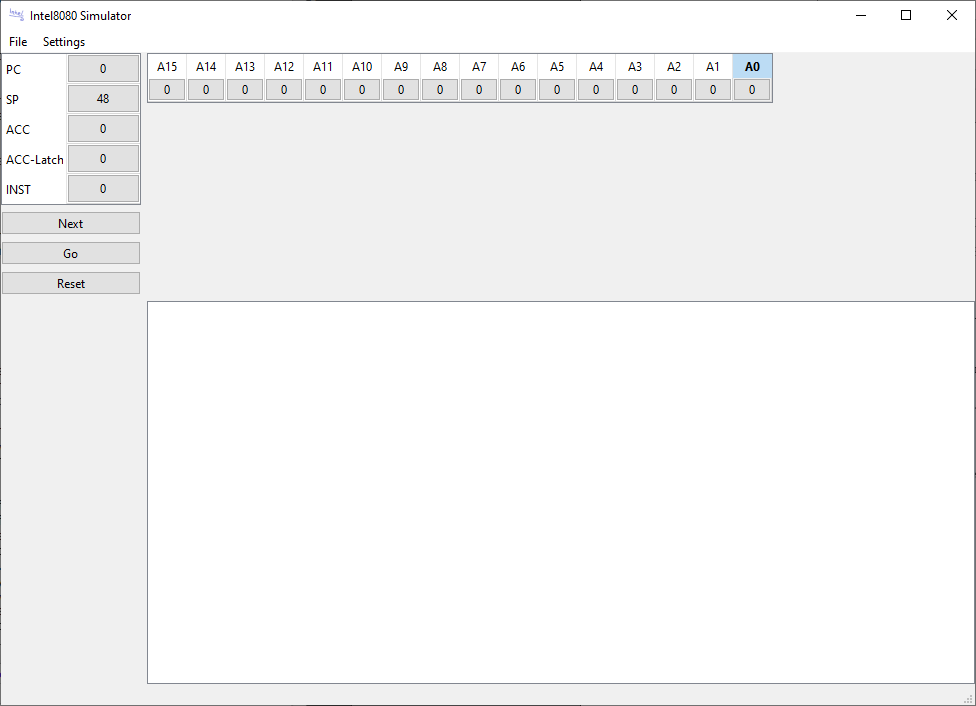
\includegraphics[width=15cm]{bilder/Intel8080_MainWindow}
\caption{Intel 8080 Simulationsfenster}
\label{fig:I8080MW}
\end{figure}

\noindent
Über das Simulationsfenster für den Intel 8080 können Programme, die aus Bytebefehlen bestehen, welche ein Intel 8080 Prozessor ausführen kann, simuliert werden. Dafür sollte (muss aber nicht) zuerst ein gültiges Programm geladen werden. Dies kann über den Menüpunkt \glqq File\grqq in der oberen Leiste getan werden (siehe Abbildung \ref{fig:LoadFile}).\imgSpaceBefore

\begin{figure}[H]
\centering
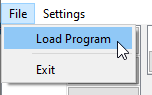
\includegraphics[width=5cm]{bilder/LoadFile}
\caption{File Menüpunkt}
\label{fig:LoadFile}
\end{figure}

\noindent
Dadurch öffnet sich ein Dateien-Explorer, über den die gewünschte Datei ausgewählt werden kann. Dabei ist zu beachten, dass in der aktuellen Version nur Ausgabedateien des verwendeten Assemblers genutzt werden können (Dateiendung \glqq .com\grqq). Über \glqq Exit\grqq kann der Benutzer ins Hauptmenü zurückkehren. Möchte man andere Programme als die mitgelieferten verwenden, so kann man den Editor der unter dem Settings Menüpunkt zu finden ist benutzen (siehe Abbildung \ref{fig:Settings}).\imgSpaceBefore

\begin{figure}[H]
\centering
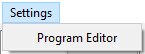
\includegraphics[width=5cm]{bilder/Settings}
\caption{Settings Menüpunkt}
\label{fig:Settings}
\end{figure}

Um die grobe Struktur eines Programms zu verstehen sind einige gültige Beispielbefehle bereits im Textfeld eingetragen (siehe Abbildung \ref{fig:ProgEdit}). Im Intel 8080 Programmers Manual sind noch weitere Beispiele für gültige Befehle aufgeführt. Das Programm kann über das untere Textfeld benannt werden. Wird der \glqq Output File\grqq-Knopf betätigt werden drei Dateien ausgegeben mit den Endungen \glqq asm\grqq, \glqq sym\grqq und \glqq com\grqq. Abhängig davon ob das Programm über die .exe-Datei gestartet wurde wird entweder der \glqq Output\grqq-Ordner verwendet oder einfach das Verzeichnis in dem die Exe ausgeführt wurde. Liegt ein Fehler vor in der Syntax wird ein Fehler ausgegeben mit dem Problem das behoben werden muss.\imgSpaceBefore

\begin{figure}[H]
\centering
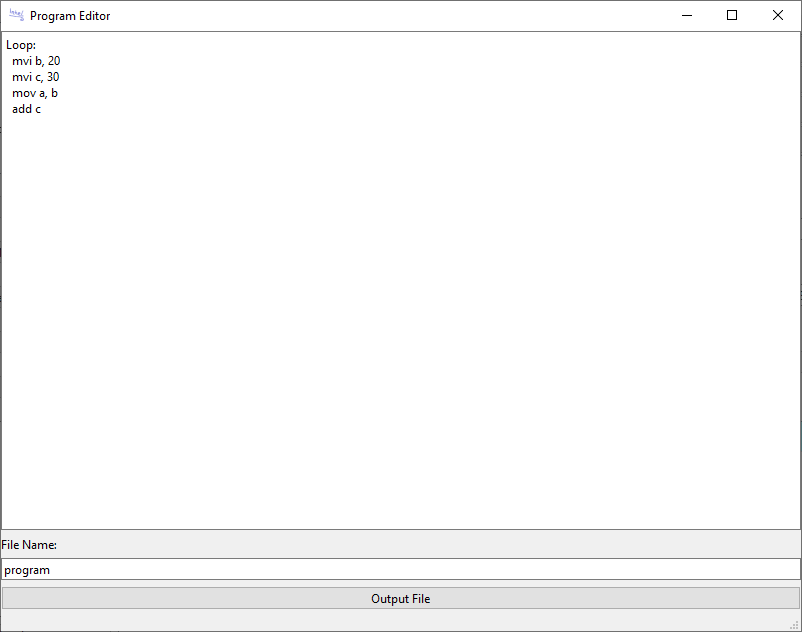
\includegraphics[width=5cm]{bilder/ProgramEditor}
\caption{Programmeditor}
\label{fig:ProgEdit}
\end{figure}

Sobald ein Programm geladen wurde, wird dieses in der dafür vorgesehenen Tabelle angezeigt (siehe Abbildung \ref{fig:ProgTable}).\imgSpaceBefore

\begin{figure}[H]
\centering
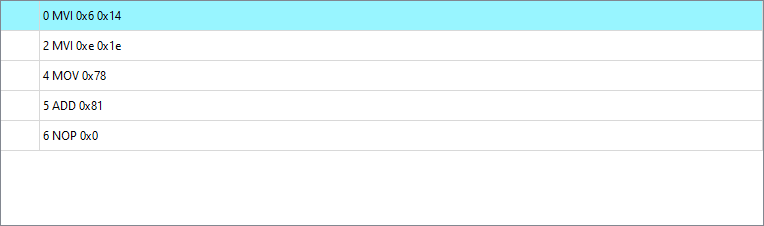
\includegraphics[width=15cm]{bilder/Program_table}
\caption{Programmtabelle}
\label{fig:ProgTable}
\end{figure}

\noindent
Dabei ist für jeden Befehl eine Zeile vorgesehen. Angezeigt werden sowohl die Position des Bytebefehls im Speicher, die Bezeichnung des Befehls, der Bytecode selbst, als auch zusätzliche Parameter, falls der jeweilige Befehl diese besitzt. Außerdem wird die Zeile, die als nächstes ausgeführt wird farbig markiert. Abgesehen von der Anzeige des Programms und des als nächste auszuführenden Befehls, ist es auch möglich, Breakpoints zu setzen (siehe Abbildung \ref{fig:Break}).\imgSpaceBefore

\begin{figure}[h]
\centering
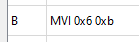
\includegraphics[width=6cm]{bilder/Breakpoint}
\caption{Breakpoint}
\label{fig:Break}
\end{figure}

\noindent
Diese werden für die automatische Ausführung des Programmes (siehe nächster Abschnitt) relevant. Wird ein Breakpoint erreicht, so stoppt das Programm, vor Ausführung des Befehls. Das Programm muss manuell fortgesetzt werden. Da vorgesehen ist, dass das gesamte Programm in dieser Tabelle angezeigt wird, ist eine Sonderbehandlung des NOP-Befehls notwendig. Dieser wird durch den Bytecode \glqq 0x00\grqq identifiziert. Bei Initialisierung des Speichers ist dies auch die Standardbelegung jedes Registers. Damit die Tabelle also nicht mit in den meisten Fällen funktionslosen NOP-Befehlen befüllt wird, musste dafür eine Ausnahmeregelung getroffen werden. Sind im Speicher zwei oder mehr NOP-Befehle direkt aufeinanderfolgend, werden diese zu einem Eintrag zusammengefasst. Da diese Tabelle lediglich das Programm in komprimierter Weise, darstellt aber keine Interaktion mit diesem ermöglicht, wurde zusätzlich das in Abbildung \ref{fig:ProgSpeicher} gezeigte Fenster in die GUI eingefügt.\imgSpaceBefore

\begin{figure}[H]
\centering
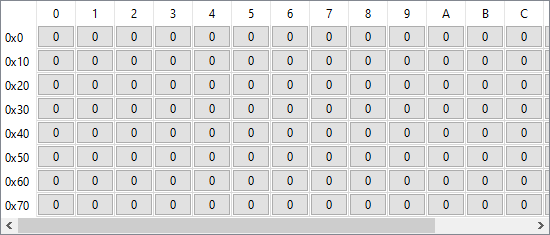
\includegraphics[width=12cm]{bilder/ProgramMemory}
\caption{Programmspeicher}
\label{fig:ProgSpeicher}
\end{figure}

\noindent
Dieses ermöglicht es, den Speicher, in Abschnitten von 128 Registern, auszulesen, wobei pro Zeile 16 Register zu sehen sind. Hierbei ist es im Gegensatz zur oben beschriebenen Tabelle möglich, diese zu bearbeiten. Dies geschieht durch klicken der entsprechenden Zelle, wodurch sich ein Dialog öffnet. Änderungen werden bei der nächsten Zustandsänderung (\glqq Next State/Machine Cycle/Instruction\grqq) in die Programmtabelle übernommen. Um auszuwählen, welche Register aus dem Programmspeicher angezeigt werden, kann das in Abbildung \ref{fig:Range} gezeigte Interface verwendet werden.\imgSpaceBefore

\begin{figure}[h]
\centering
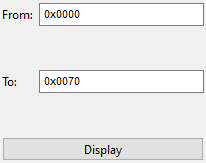
\includegraphics[width=6cm]{bilder/Range}
\caption{Range Einstellungen}
\label{fig:Range}
\end{figure}

\noindent
Hiermit kann der Start- oder Endwert des angezeigten Registerblocks eingestellt werden. Wird einer der beiden Werte verändert, ergänzt sich der andere automatisch, um den angezeigten Satz von 128 Registern konstant zu halten. Der Abstand muss dabei immer genau 128 Register sein. Eingetragene Werte müssen außerdem immer ein Vielfaches von sechzehn sein, da dies der Anzahl an Registern einer Zeile entspricht. Die Ausführung des Programms wird über fünf Knöpfe im Simulationsfenster gesteuert (siehe Abbildung \ref{fig:Bedienen}).\imgSpaceBefore

\begin{figure}[H]
\centering
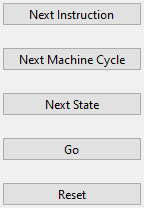
\includegraphics[width=6cm]{bilder/Bedienen}
\caption{Bedien-Knöpfe zur Ausführung des Programmes}
\label{fig:Bedienen}
\end{figure}

\noindent
Über \glqq Next Instruction\grqq wird der nächste Befehl, der in der Programmtabelle farbig hervorgehoben ist, ausgeführt und die Benutzeroberfläche wird entsprechend aktualisiert. Dasselbe gilt für \glqq Next Machine Cycle\grqq und für \glqq Next State\grqq, wobei diese jeweils nur den nächsten Machinenzyklus oder den nächsten Zustand ausführen. Über \glqq Go\grqq wird automatisch das Programm ausgeführt. Bei erneutem Drücken wird das Programm pausiert. \glqq Reset\grqq setzt den Simulator auf die Ausgangssituation zurück, behält aber den aktuellen Zustand des Programmspeichers bei. Es ist auch möglich, einzelne Register des Prozessors auszulesen. Wie in Abbildung \ref{fig:Register} zu sehen ist, werden diese mit ihren entsprechenden Bedeutungen und Werten angezeigt.\imgSpaceBefore

\begin{figure}[h]
\centering
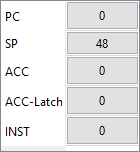
\includegraphics[width=4cm]{bilder/Register}
\caption{Ausgewählte besondere Register}
\label{fig:Register}
\end{figure}

\noindent
Die gezeigten Einträge stehen für:\imgSpaceBefore

\begin{itemize}
	\item PC: Program Counter Register
	\item SP: Stack Pointer Register
	\item ACC: Accumulator Register
	\item ACC-Latch: Accumulator-Latch Register
	\item INST: Instruction Register
\end{itemize}

\noindent
Durch Klicken auf die entsprechende Werte lassen sich diese in einem neuen Fenster bearbeiten.
Das in Abbildung \ref{fig:GenReg} gezeigte Modul zeigt die restlichen Register an.\imgSpaceBefore

\begin{figure}[h]
\centering
\begin{subfigure}{.5\textwidth}
  \centering
  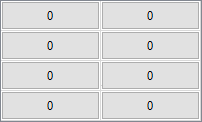
\includegraphics[width=.7\linewidth]{bilder/GenericRegister_sim}
  \caption{Simulator generische Register}
  \label{fig:GenReg_s}
\end{subfigure}%
\begin{subfigure}{.5\textwidth}
  \centering
  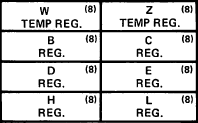
\includegraphics[width=.7\linewidth]{bilder/GenericRegister_pic}
  \caption{Äquivalente Darstellung}
  \label{fig:GenReg_p}
\end{subfigure}
\caption{Simulator Register und Darstellung}
\label{fig:GenReg}
\end{figure}

\noindent
Damit gemeint sind die generischen Register ohne feste Funktion, welche jeweils eine Speicherkapazität von acht Bit haben. Über die in Abbildung \ref{fig:Interrupt} dargestellte Funktion ist es möglich, ein Interrupt mit einem gültigen Interrupt-Bytevektor auszulösen.\imgSpaceBefore

\begin{figure}[h]
\centering
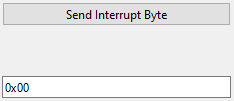
\includegraphics[width=6cm]{bilder/Interrupt}
\caption{Bereich zum Senden eines Interrupts}
\label{fig:Interrupt}
\end{figure}

\noindent
Dabei wird geprüft, ob die Operation gültig ist. Ist die der Fall, wird sie beim nächstmöglichen Zustand berücksichtigt und ausgeführt. Ist die Operation ungültig, wird eine Fehlermeldung ausgegeben.
\newpage
\noindent
Die letzte Funktionalität der Benutzeroberfläche ist ein Log in dem die einzelnen Operationen aufgelistet werden, die in jedem Zustand vorgenommen werden (siehe Abbildung \ref{fig:Logger}).\imgSpaceBefore

\begin{figure}[h]
\centering
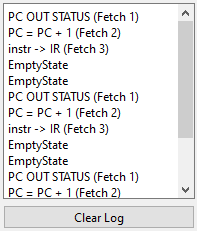
\includegraphics[width=6cm]{bilder/Logger}
\caption{Zustands-Log für aufeinanderfolgende NOP-Befehle}
\label{fig:Logger}
\end{figure}

\noindent
Über den darunterliegenden \glqq Clear Log\grqq-Knopf lässt sich der Inhalt des Logs löschen. Bei Laden eines neuen Programms wird der Log ebenfalls geöscht. Ein nicht mehr in der finalen Version der GUI vorhandenes Register, welches dem Nutzer angezeigt wird und welches bearbeitet werden kann ist in Abbildung \ref{fig:AddBuff} zu sehen.\imgSpaceBefore

\begin{figure}[h]
\centering
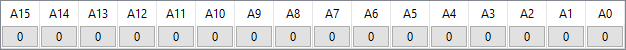
\includegraphics[width=15cm]{bilder/AddBuff}
\caption{Adresspuffer}
\label{fig:AddBuff}
\end{figure}

\noindent
Gezeigt ist der Adresspuffer, welcher für das Auswählen von externen Geräten über das Bussystem zuständig ist. Die Darstellung wurde hier bitweise gewählt, das heißt, statt die ganzen 2 Byte des Registers zu bearbeiten, werden die einzeln Bits angesteuert.

\newpage

\subsection{Tutorial}
Das Tutorial für die Handhabung des Simulators ist über das Hauptmenü erreichbar. Es besteht aus fünf verschiedenen Bildern, welche jeweils die einzelnen Elemente des Simulators zeigen und deren Funktion näher beschreiben (siehe Abbildung \ref{fig:Tutorial}).\imgSpaceBefore

\begin{figure}[h]
\centering
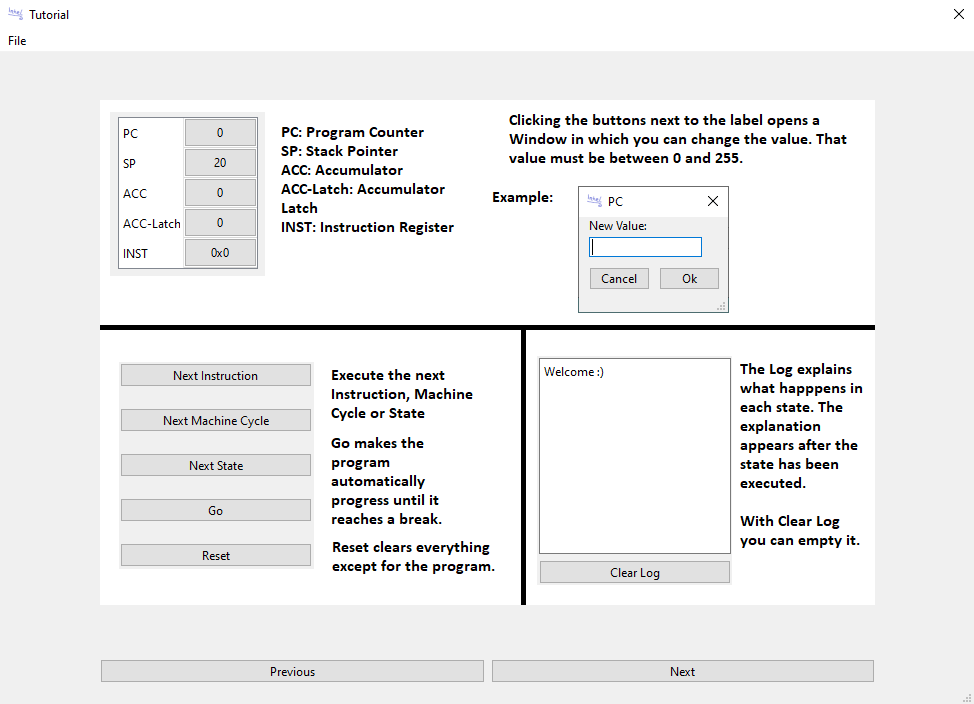
\includegraphics[width=15cm]{bilder/Tutorial}
\caption{Tutorial-Fenster}
\label{fig:Tutorial}
\end{figure}

\noindent
Um zum nächsten bzw. vorherigen Bild zu wechseln werden die zwei unteren Knöpfe verwendet. Der Text wurde wie der Rest der Simulatoroberfläche in Englisch verfasst.

\newpage

\section{Implementierung}
Von Andreas\\

\noindent
Es wurde ein Simulator eines 8-Bit-Prozessors geschrieben.
Der 8-Bit-Prozessor wurde mit einer Software mit graphischer Oberfläche realisiert. Diese zeigt dem Benutzer den aktuellen Zustand des Prozessors (Intel 8080) an. Der Simulator unterstützt alle Befehle des realen Prozessors und kann Interrupts ausführen. Lediglich der Single-Prozessor-Simulator ist in der Lage auch einen Interrupt durch die GUI zu generieren.


\subsection{Multi-Prozessor-Simulator}
Mit diesem Simulator soll es möglich sein, zuvor assemblierten Code auszuführen. Dafür wird ein Assembler \cite{Assembler} verwendet, der aus dem Source Code (.asm) eine .com-Datei erstellt. Aus dieser kann das komplette Programm ausgelesen werden. Zusätzlich dazu wird noch eine Datei (.sym) erstellt, die die Labels/Sprungmarken abspeichert. Dieser Assembler wurde mit in den Simulator integriert. Diese Version des Simulators verfügt über keine GUI, deshalb muss dem Prozessor der Assemblercode in der Source-Datei (Intel8080.py) übergeben werden. Der Prozessor leitet den Code zum Assembler weiter und liest das Ergebnis in seinen Programmspeicher ein. 
Zuallererst wurde der Intel 8080 implementiert. Dieser wurde voll-funktionsfähig implementiert, bevor damit begonnen wurde, andere Prozessoren zu implementieren. Im Zuge der Recherche ergab sich, dass sich die Prozessoren nur minimal unterscheiden, deshalb wurde sich dafür entschieden einen Prozessor genauer zu simulieren. Die Beschreibung dieses Simulators kann auf Seite \pageref{SPS_impl} gefunden werden.


\subsubsection{Programmablauf}
Der eigentliche Simulator verwendet nur die .com-Dateien. Zuallererst wird die .com-Datei ausgelesen und in den Programmspeicher des Prozessors geschrieben. Um den ersten Befehl ausführen zu können, wird zuerst nur ein Byte aus dem Programmspeicher, an der Stelle des Programmzählers, eingelesen. Danach wird das erste Byte dekodiert.
Je nach Befehl werden noch weitere Bytes eingelesen, die für den eigentlichen Befehl benötigt werden. Sobald alle nötigen Informationen eingelesen wurden, wird der Befehl ausgeführt. Jeder Befehl muss entsprechend den Programmzähler anpassen, damit der nächste Befehl wieder korrekt eingelesen werden kann. Mit diesem Simulator ist es auch möglich, Interrupts auszulösen. Vor der Ausführung eines Befehls wird geprüft, ob ein Interrupt ausgelöst wurde. Ist das der Fall, wird das Interrupt-Byte ausgewertet und ausgeführt. Normalerweise wird dieses Byte von dem Interrupt-Erzeuger mitgeschickt. Meistens ist dies ein Reset-Befehl, der an eine von acht Stellen springt und die dort liegenden Befehle ausführt. Mit 3 Bits kann damit entschieden werden, wo die Subroutine beginnen soll (Byte 0, 8, 16 ... 56). Es ist aber auch möglich, dass ein anderer, ein Byte langer Befehl übergeben und direkt ausgeführt wird.


\subsubsection{Dekodieren eines Befehls}
\noindent
Um aus einem Byte einen Befehl analysieren zu können, wird dieser Wert mit vielen Hexadezimalwerten verglichen. Anhand der Dokumentation des Intel 8080 werden somit alle Befehle unterschieden.
Wie in  Abbildung \ref{fig:ReadInstruction} zu sehen ist, wird der Befehl \glqq Add Immediate to A with carry (ACI)\grqq\ mit dem Wert 0xCE assoziiert.
Bei vielen Befehlen wie ACI wird auf genau einen Wert geprüft. Es gibt aber auch andere Befehle, wobei nicht alle Bits des Bytes den Befehl beschreiben. In Abbildung \ref{fig:ReadInstruction} ist zu sehen, dass der Befehl \glqq Add Memory to A with carry (ADC)\grqq\ nicht so einfach verglichen wird. Bei diesem Befehl werden in den letzten drei Bits des Befehlsbytes das 8-Bit-Register kodiert, welches verwendet werden soll. Deshalb wird die Instruction-Variable zuerst mit dem Wert 0xF8 bitweise verUNDet, damit die letzten drei Bit ignoriert werden. Somit werden alle Bitkombinationen erkannt, bei denen die ersten fünf Bits mit dem Wert 0x88 übereinstimmen. Wenn dann bekannt ist, dass es sich um einen ADC-Befehl handelt, wird das Register ermittelt, das verwendet werden soll. Dies geschieht über die get\_reg8d\_from\_inst(instruction)-Methode. Für die unterschiedlichen Fälle, der Register-Kodierung, gibt es jeweils eine eigene Methode. Diese liefert einen Wert zwischen 0 und 8, entsprechend der Abbildung \ref{fig:register_kodierung}.\imgSpaceBefore

\begin{figure}[h]
\centering
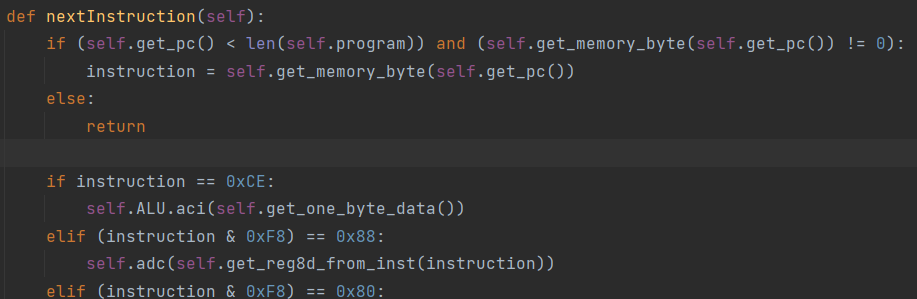
\includegraphics[width=10cm]{Bilder/ReadInstruction}
\caption{Funktion für das Lesen und Dekodieren eines Bytes}
\label{fig:ReadInstruction}
\end{figure}

\noindent
Dieses Vorgehen wird bei einigen Befehlen verwendet. In Kapitel \ref{chapter:opcode} wird genauer gezeigt, wie die Register in den Befehlen kodiert werden.


\subsubsection{Programmaufbau}
\label{chapter:MPS_aufbau}

Der Simulator besteht hauptsächlich aus drei Klassen:

\begin{itemize}
\item Dem Prozessor (Intel8080.py)
\item Der ALU (Intel8080\_ALU.py)
\item Den Register (Intel8080\_Registers.py)
\end{itemize} 

\noindent
Die Register-Klasse ist hauptsächlich als Datenspeicher gedacht und besitzt keine spezielle Methoden. In der Prozessor- und der ALU-Klasse werden Befehle ausgeführt. Es werden zwei Arten von Befehlen unterschieden. Befehle wie Sprungbefehle, die die ALU nicht benötigen und Befehle wie Additionen, die die ALU verwenden. 
Die Befehle, die die ALU nicht verwenden, wurden in in der Intel8080.py implementiert, die restlichen entsprechend in der ALU. Jeder Befehl wird durch eine eigene Methode implementiert. Somit kann ein Befehl schnell gefunden und angepasst werden. In diesen Methoden läuft der komplette Befehl ab. Somit werden in diesen Methoden auch weitere Bytes eingelesen, die für die Ausführung des Befehls notwendig sind.
Bei jedem Lesevorgang aus dem Programmspeicher wird der Programmzähler automatisch um eins erhöht. Deshalb ist es nicht möglich das gleiche Byte mehrfach hintereinander zu lesen. Um das gleiche Byte nochmal lesen zu können, müsste der Programmzähler manuell angepasst werden.

\imgSpaceBefore
\begin{figure}[h]
\centering
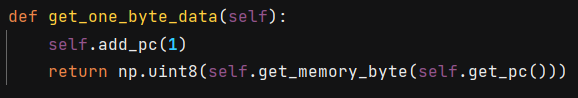
\includegraphics[width=15cm]{Bilder/GetOneByteData}
\caption{Implementierung des Lesens eines Bytes}
\label{fig:GetOneByteData}
\end{figure}

\noindent
Der Befehl DCX reduziert das angegebene 16-Bit Register um eins. Abbildung \ref{fig:dcx_impl} zeigt die Implementierung des DCX-Befehls.
Dort ist zu sehen, dass es bei den 16-Bit Registern eine grundlegende Unterscheidung gibt. Es gibt einen Fall für den Stackpointer und einen für die anderen 16-Bit Register, die aus zwei 8-Bit Registern zusammengesetzt werden. Mittels des übergebenen Parameters \glqq rp\grqq\ kann ermittelt werden ob es sich um den Stackpointer (rp  == 3 bedeutet Stackpointer) handelt, der angepasst werden soll.
Der Stackpointer kann einmal ausgelesen, um 1 reduziert, und dann wieder in sein Register gespeichert werden.
Bei den zusammengesetzten 16-Bit Registern, werden zuerst beide 8-Bit Register ausgelesen und dann zusammengebaut. Dieses Ergebnis kann dann um 1 reduziert werden. Danach wird der 16-Bit Wert wieder aufgetrennt und in die 8-Bit Register gespeichert. 

\imgSpaceBefore
\begin{figure}[H]
\centering
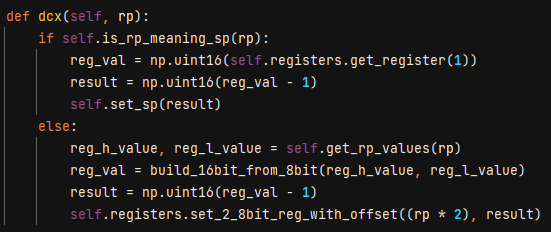
\includegraphics[width=15cm]{Bilder/dcx_impl}
\caption{Implementierung des DCX-Befehls}
\label{fig:dcx_impl}
\end{figure}

\noindent
Die zusammengesetzten Register können alle gleich behandelt werden, da bei dem Programmkonzept beachtet wurde, dass dies öfter vorkommen kann. Deshalb wurden die Register so positioniert, dass auf die Register anhand ihrer Kodierung (siehe Abbildung \ref{fig:register_kodierung}) direkt zugegriffen werden kann. Ebenso liegt damit das High Byte eines 16-Bit Registers einen Platz vor dem Low Byte. Mit dieser Anordnung kann mittels einfacher mathematischer Berechnungen die entsprechende Array-Stelle ermittelt werden. So kann aus einem rp-Wert (0-2) das entsprechende Array-Feld (High Byte) mittels einer Multiplikation mit 2 und der Addition eines Offsets berechnet werden. Um auf das Low Byte zu kommen, muss dann nur noch 1 addiert werden.

\imgSpaceBefore
\begin{figure}[H]
\centering
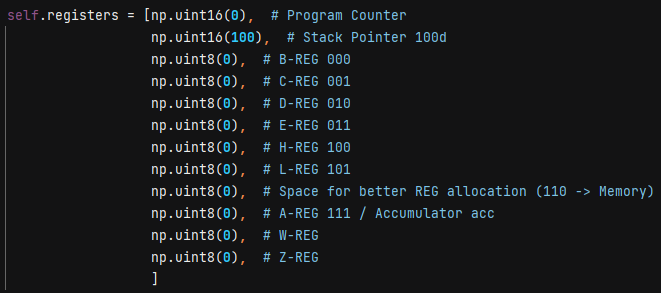
\includegraphics[width=15cm]{Bilder/register_array}
\caption{Register Array des Intel 8080}
\label{fig:reg_array}
\end{figure}


\noindent


\subsubsection{Befehlsvarianten}

Der Intel 8080 kennt mehrere Befehle, die sowohl eine direkte als auch eine indirekte Variante besitzen. Der Unterschied liegt darin, dass die verrechneten Werte, aus unterschiedliche Stellen geladen werden. Aus diesem Grund greifen beide Befehle im Hintergrund auf die gleichen Methoden zu. Somit ist sicher gestellt, dass bei Bedarf nur eine Stelle im Quellcode angepasst werden muss.
\\
Ein Beispiel dafür ist die \glqq Subtract register/immediate from A with borrow (SBB/SBI)\grqq. Es gibt zwar für beide Mnemonics eine Methode in der Intel8080-Klasse, die Methode von SBB leitet aber später in der ALU-Klasse nur noch auf die SBI-Methode weiter.

\imgSpaceBefore
\begin{figure}[h]
\centering
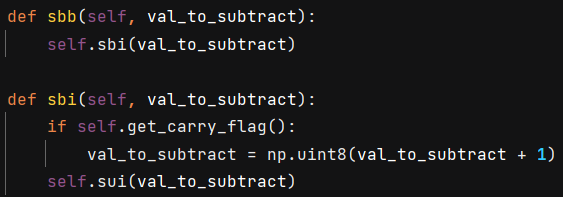
\includegraphics[width=15cm]{Bilder/DoubleUsedMethodSubtract}
\caption{Zugrundeliegende Implementierung von SBB und SBI}
\label{fig:DoubleUsedMethodSubtract}
\end{figure}

\noindent
Die direkten Befehle lesen dabei das zweite Byte, das zu diesem Befehl gehört und rufen die
Methode SBI in der ALU-Klasse auf. Für indirekte Befehle wie SBB wird zuerst in der Intel8080-Klasse noch der Wert aus dem Speicher gelesen. Dieser wird deshalb gelesen, da die ALU keinen direkten Zugriff auf den Speicher hat. Mit dem gelesenem Wert wird dann in der ALU-Klasse die SBB-Methode aufgerufen. Diese leitet innerhalb der Klasse nur noch auf die SBI Methode weiter.
\\\\
Die Sprungbefehle werden ähnlich behandelt. Für diese gibt es mehrere Varianten, die aber nur auf unterschiedliche Flags reagieren. Deshalb wurde auch dort eine zugrundeliegende Methode geschrieben, auf die alle anderen verweisen. So wird nur für die spezifische Varianten das verwendete Flag weitergegeben.  Abbildung \ref{fig:JumpVariants} zeigt wie bei dem Jump-on-Carry Befehl vorgegangen wird. So ruft die jc-Methode die jump\-on-Methode mit dem Carry-Flag auf. In der jump\_on-Methode werden immer die nächsten zwei Bytes gelesen, die die Adresse beinhaltn, auf die gesprungen werden soll. Nur sofern das übergebene Flag gesetzt ist wird der Sprung ausgeführt andernfalls wird das Programm normal weitergeführt.

\imgSpaceBefore
\begin{figure}[H]
\centering
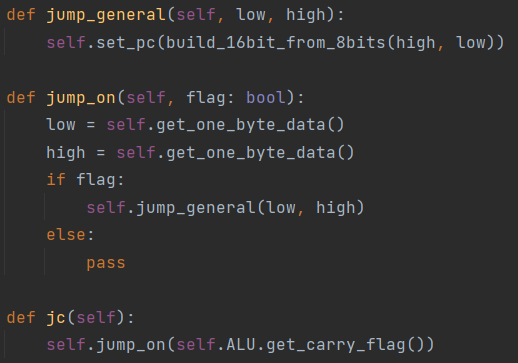
\includegraphics[width=10cm]{Bilder/JumpVariants}
\caption{Implementierung der Sprungbefehle}
\label{fig:JumpVariants}
\end{figure}


\subsubsection{Binäre Addition und Subtraktion}
Da die Additions- und Subtraktionsbefehle das Carry- und Auxiliary-Carry-Flag verändern, musste eine manuelle Addition implementiert werden. Diese ist in Abbildung \ref{fig:binaere_addition} zu sehen. Das Carry-Flag, das anzeigt, ob ein Überlauf beim siebten Bit stattgefunden hat, hätte noch ohne eine eigene Implementierung der Addition funktioniert. Dafür müsste vor dem Casten in einen 8-Bit Wert überprüft werden, ob der Wert größer als 255 ist. Da aber zusätzlich noch das Auxiliary-Carry-Flag beachtet werden musste, das einen Überlauf von Bit 3 anzeigt, wurde die Addition selber implementiert. Diese Implementierung liefert das Carry-, Auxiliary-Carry-Flag und das Ergebnis der Addition. Somit können die Flags korrekt gesetzt werden, sofern die Befehle diese Flags ändern. Wird eines der beiden Flags verändert, wird darauf zurückgegriffen. Der INX-Befehl, der einen 16-Bit Wert um 1 erhöht, verändert aber keine Flags, weshalb dort eine normale Addition durchgeführt wird.

\imgSpaceBefore
\begin{figure}[H]
\centering
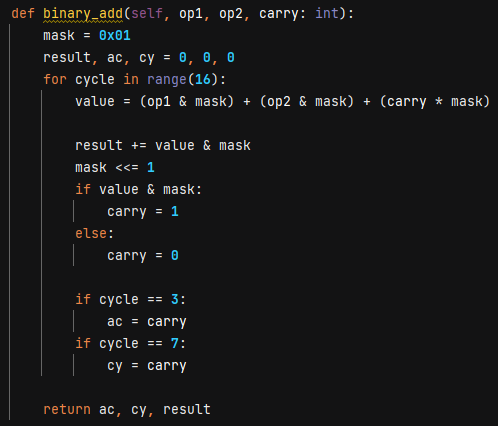
\includegraphics[width=10cm]{Bilder/binaere_addition}
\caption{Implementierung der binären Addition}
\label{fig:binaere_addition}
\end{figure}

\subsection{Single-Prozessor-Simulator}
\label{SPS_impl}

\noindent
In diesem Kapitel werden die Funktionen der aktuellen Version des Simulators beschrieben. Dieser unterscheidet sich insofern von dem Multi-Prozessor-Simulator, dass jeder Befehl aus mehreren Maschinenzyklen und diese wiederum aus mehreren Zuständen bestehen. So ist es möglich, komplette Befehle aber auch einzelne Maschinenzyklen oder sogar Zustände auszuführen. Damit kann wesentlich besser nachvollzogen werden, wie ein Prozessor tatsächlich funktioniert. In der Multi-Prozessor-Variante konnten zwar Programme ausgeführt werden, aber der Ablauf der Befehlsausführung unterschied sich deutlich von der Funktionsweise eines realen Prozessors.

\subsubsection{Aufbau eines Befehls}

Jeder Befehl besteht aus einem Array von Maschinenzyklen. Zusätzlich enthält jeder Befehl auch einen Zähler, wie viele Maschinenzyklen der Befehl schon ausgeführt hat. Ein Befehl hat auch nur eine Methode, die zur Ausführung des Befehls notwendig ist. Die next\_state()-Methode des Befehls sorgt dafür, dass der aktuelle Maschinenzyklus seine next\_state()-Methode ausführt. Wenn die Maschinenzyklus next\_state()-Methode True zurückliefert, bedeutet das, dass der letzte Zustand des Maschinenzyklus ausgeführt wurde. Wenn dies der Fall ist, wird der Maschinenzyklus Zähler um eins erhöht und es wird ebenfalls ein True zurückgeliefert. Dieses Signal des Maschinenzyklus wird bis in die äußerste Schicht, die GUI, weitergeleitet, damit dort spezielle Ereignisse ausgeführt werden können. Beim nächsten Aufruf von next\_state() wird somit der erste Zustand des nächsten Maschinenzyklus ausgeführt.
\\

\noindent
Jeder Maschinenzyklus besteht aus einem Array von Zuständen, einem Zähler, der die bisher ausgeführten Zustände zählt und einer Referenz auf den Prozessor. Diese Referenz ist notwendig, damit die Zustände, die in den Maschinenzyklen ausgeführt werden, den Prozessor verändern und dessen Methoden verwenden können. Die next\_state()-Methode führt immer die run()-Methode der Zustände aus und erhöht seinen Zähler um eins. Wenn der eben ausgeführte Zustand der letzte im Maschinenzyklus war, wird der Zähler zurückgesetzt und ein True zurückgegeben.
\\

\noindent
Ein Zustand besitzt nur eine Referenz zum Prozessor und eine run()-Methode, die den Zustand ausführt. Da ein Zustand zu allen möglichen Stellen in einem Maschinenzyklus verwendet werden kann, besitzt der Zustand selber keine weiteren Informationen.


\subsubsection{Programmablauf}

Wie bei der Multi-Prozessor-Version dieses Simulator wird eine .com-Datei zur Ausführung des Programms benötigt. Über die GUI kann eine solche Datei eingelesen werden. Damit wird wieder der Programmspeicher befüllt.
Die GUI besitzt vier Knöpfe, die das ausführen eines Befehls/Maschinenzyklus oder Zustand auslöst. Bei dem \glqq Next State\grqq\ -Knopf wird genau ein Zustand ausgeführt. Bei dem \glqq Next Machine Cycle\grqq\ -Knopf wird der aktuelle Maschinenzyklus bis zum Schluss ausgeführt. Der  \glqq Next Instruction\grqq\ -Knopf verhält sich wie der Maschinenzyklus-Knopf. Der \glqq Go\grqq\ -Knopf führt zu solange den nächsten Zustand aus bis der Knopf wieder gedrückt wird. Die drei ersten Knöpfe sind auf eine Methode in der Intel8080-Klasse gebunden, die den selben Namen tragen wie der Knopf. Jeder dieser Methoden gibt True zurück, wenn der nächste auszuführende Zustand zu einem neuen Befehl gehört.
Die next\_instruction()-Methode führt solange die next\_machine\_cycle()-Methode aus, bis diese True zurückliefert. Diese wiederum führt solange die next\_state\_internal()-Methode aus, bis diese True zurückliefert. Diese liefert True, wenn der letzte Zustand eines Maschinenzyklus ausgeführt wurde. Die next\_state()-Methode ruft nur einmal die next\_state\_internal()-Methode auf.

\noindent
Die next\_state\_internal()-Methode, steuert wann ein neuer Befehl dekodiert und eine neue Klasse geladen werden muss. Wenn der nächste Zustand der erste eines neuen Befehls ist, wird der current\_instruction-Variable ein NOP-Befehl zugewiesen. Da bei allen Befehlen die ersten drei Zustände die gleichen sind, ist es unbedeutend, welcher Befehl hier geladen wird. Erst im dritten Zustand wird der tatsächliche Befehl geladen. Von diesem Befehl wird der zuletzt ausgeführte Zustand auf drei gesetzt. Wenn der letzte Zustand eines Maschinenzyklus ausgeführt wurde, wird True zurückgegeben. Wenn ein Befehl frühzeitig abgebrochen werden soll, z.B. bei einem bedingten Sprung, wird das ebenfalls hier gesteuert.

\subsubsection{Dekodieren eines Befehls}
Bei jedem Fetch-Zyklus wird das aktuelle Befehlsbyte in die cpu\_instruction\_register-Variable geschrieben. Ähnlich wie bei der Multi-Prozessor-Version, wird beim Dekodieren dieses Byte mit Hexadezimalen Werten verglichen. Bei dieser Version wird beim Dekodieren aber unterschieden zwischen Befehlen, die entweder ein Register oder eine Adresse als Parameter erhalten (siehe Abbildung \ref{fig:Decode_instr}). Dies ist deshalb wichtig, da sich die Maschinenzyklen davon unterscheiden. Abbildung \ref{fig:ReadInstruction}  zeigt, dass in der ersten Version für alle ADD-Befehle nur eine Methode aufgerufen wird. Damit der Prozessor die richtigen Klassen zur Ausführung verwendet, wird in der current\_instruction-Variable ein Objekt des richtigen Befehls gespeichert.

\imgSpaceBefore
\begin{figure}[H]
\centering
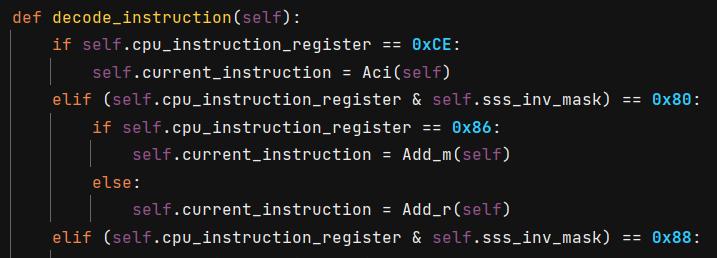
\includegraphics[width=15cm]{bilder/DecodeInstruction}
\caption{Implementierung der Dekodierung}
\label{fig:Decode_instr}
\end{figure}

\subsubsection{Programmaufbau}

Der Simulator besteht, wie der Multi-Prozessor-Simulator, immer noch hauptsächlich aus dem Prozessor, der ALU und den Registern. Durch die Verwendung eigener Klassen für Befehle, Maschinenzyklen und Zustände, gibt es nun wesentlich mehr Klassen. Insgesamt werden

\begin{itemize}
\item 74 Befehls-Klassen,
\item 85 Maschinenzyklen-Klassen, und
\item 101 Zustands-Klassen
\end{itemize}

\noindent
verwendet. Zusätzlich dazu gibt es noch ungefähr 13 Klassen, von denen die oben genannten abgeleitet sind.

\noindent
Der in Kapitel \ref{chapter:MPS_aufbau} gezeigte DCX-Befehl sieht nun folgendermaßen aus.

\imgSpaceBefore
\begin{figure}[H]
\centering
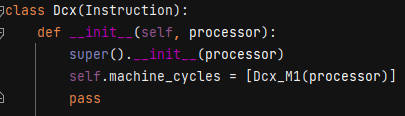
\includegraphics[width=10cm]{bilder/dcx_inst}
\caption{DCX-Befehl}
\vspace{15pt}
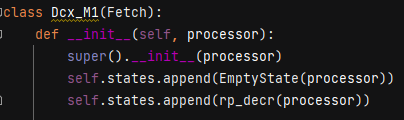
\includegraphics[width=10cm]{bilder/dcx_mc}
\caption{DCX-Maschinenzyklus}
\label{fig:Dcx_instr}
\end{figure}

\noindent
Bei vielen Befehlen werden leere Zustände verwendet. Das kommt daher, dass es mit dem Simulator momentan nicht möglich ist, einen Zustand zu erstellen, der zwei Takte dauert. Deshalb wird mit dem ersten Takt ein leerer Zustand ausgeführt und im zweiten dann erst der eigentliche Zustand. Somit werden die Daten zur gleichen Zeit in die Register/Speicher geschrieben, wie es bei einem realen Prozessor auch der Fall ist.

\imgSpaceBefore
\begin{figure}[H]
\centering
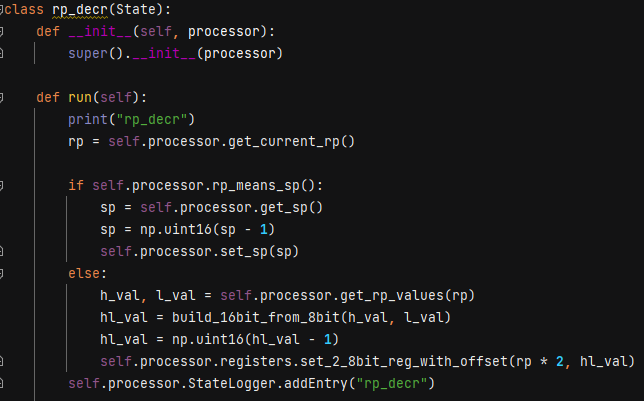
\includegraphics[width=14cm]{bilder/dcx_state}
\caption{DCX (rp\_decr) Zustand}
\label{fig:Dcx_state}
\end{figure}

\noindent
Da der DCX-Befehl nur aus einem Maschinenzyklus besteht und mit dem leeren Zustand nur über einen Zustand verfügt, der den Befehl ausmacht, werden im Folgenden anderen Befehle gezeigt, die diese Klassenstruktur besser veranschaulichen. Diese Beispiel sollen auch verdeutlichen , wie Befehle des gleichen Typs auf die selben Maschinenzyklen und Zustände zurückgreifen.

\subsubsection{Testing}
Um sicherzustellen, dass alle Befehle korrekt ausgeführt werden, wurden Tests erstellt. 
Speziell wurden Integrationstests geschrieben, um zu kontrollieren, dass dies der Fall ist und die Zustände sehr simpel aufgebaut sind. Abbildung \ref{fig:test_aci} zeigt wie einer der Tests aufgebaut ist. 

\imgSpaceBefore
\begin{figure}[H]
\centering
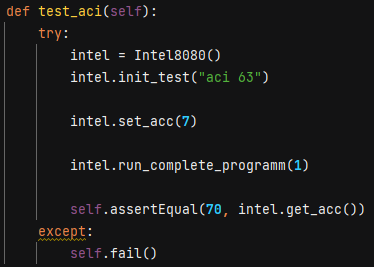
\includegraphics[width=8cm]{bilder/test_aci}
\caption{Test für den ACI-Befehl}
\label{fig:test_aci}
\end{figure}

\noindent
Zuerst wird ein Intel8080-Prozessor-Objekt (ohne GUI) erzeugt. Mit intel.init\_test() wird die Zeichenkette zuerst assembliert und dann in den Programmspeicher geschrieben. In diesem Fall wird zu Vorbereitung der Wert 7 in den Akkumulator geschrieben. Mit intel.run\_complete\_programm() führt der Simulator so viele Befehle aus wie durch den Zahlenwert übergeben. Dies ist notwendig, wenn z.B. mit Labels gearbeitet wird und diese nicht auf die Adresse 0 verweisen sollen. Nach der Ausführung des Befehls wird überprüft, ob der Wert im Akkumulator der korrekte ist. Sofern irgendwo ein Fehler auftaucht, gilt der Test als gescheitert.
\\

\noindent
Mit dem obigen Test wurde geprüft ob der Ergebniswert der zu erwartende ist. Da manche Befehle  von Flags abhängig sind und diese teilweise auch verändern, gibt es noch andere Tests, um dies zu kontrollieren. Nicht jeder Befehl wird so ausgiebig getestet wie der ADC-Befehl (siehe \ref{fig:test_adc}). Da der ADC r, der ADC m und der ACI-Befehl aus dem ADC\_MC-Maschinenzyklus bestehen, wird nur einer dieser Befehle besonders stark getestet. Wenn ein anderer Zustand eines Befehls nicht korrekt wäre, würde sehr wahrscheinlich der einfache Test für einen, wenn nicht sogar mehrere, einen Fehler anzeigen. Somit wird mit mehreren weiteren Tests für den Maschinenzyklus hauptsächlich die sich verändernden Flags getestet.

\imgSpaceBefore
\begin{figure}[H]
\centering
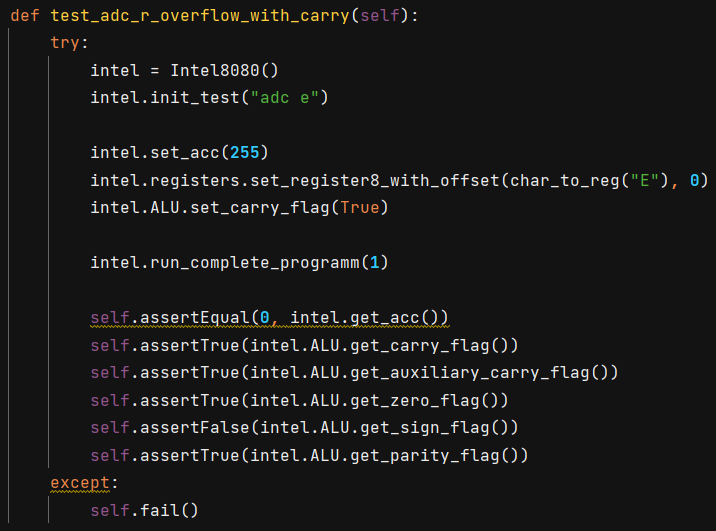
\includegraphics[width=10cm]{bilder/test_adc}
\caption{einer von mehreren Tests für den ADC-Befehl}
\label{fig:test_adc}
\end{figure}

\noindent
In diesem Test (Abbildung \ref{fig:test_adc}) wird überprüft, ob sich die Flags korrekt verhalten, wenn ein Überlauf stattfindet. Ebenso wird hier auch noch mal getestet, ob das Carry-Flag mit in die Berechnung einfließt. Deswegen wird vor dem Befehl das Carry-Flag gesetzt. Da dieser ADC r Befehl auf ein Register zugreift, muss dieses auch vor dem Test noch befüllt werden. Nach der Ausführung des Programms werden alle Flags ausgewertet. Sofern nur eines davon nicht den korrekten Wert enthält, wird der Test als nicht bestanden markiert.


\subsubsection{Befehlsvarianten}
Alle Befehle haben die gleichen ersten drei Zustände. Aus diesem Grund wurde ein Fetch-Maschinenzyklus erstellt, von dem jeder erste Maschinenzyklus abgeleitet wurde. Der RST-Befehl hat, als einzige Ausnahme, einen anderen dritten Zustand. Normalerweise wird im dritten Zustand nur der aktuelle Befehl in das Befehls Register geschrieben. Beim RST-Befehl wird aber zusätzlich noch das W-Register auf Null gesetzt. Dies ist deswegen wichtig, da der Befehl an eine von acht Programmstellen springen soll. Diese liegen alle am Anfang des Programmspeichers und benötigen deswegen ein leeres W-Register. Für Sprünge werden das W- und Z-Register verwendet. In den Maschinenzyklen 2-4 wird aber nur das Z-Register auf den entsprechenden Wert gesetzt.
\\

\noindent
Bei einigen Befehlen gibt es grundsätzlich drei verschiedene Typen, die unterschieden werden. Einen direkten Befehl, der ein weiteres Byte hinter dem Befehl im Programmspeicher liest, einen Befehl, der einen Register-Wert liest, im folgenden als Register-Befehl bezeichnet, und einen Befehl, der zuerst die zwei folgenden Bytes aus dem Programmspeicher liest, daraus eine Adresse bildet und dann an diese Adresse springt und den dort liegenden Wert verwendet, im restlichen Kapitel an Speicher-Befehl bezeichnet.

\imgSpaceBefore
\begin{table}[H]
\centering
\begin{tabular}{|l c c c|c| } 
 \hline
 Beschreibung & Register-Befehl & Speicher-Befehl & Direkter Befehl \\
 \hline 
 Addition mit Acc & ADD r & ADD m & ADI \\ 
 Addition mit Acc \& Cy & ADC r & ADC m & ACI \\ 
 Subtraktion mit Acc & SUB r & SUB m & SUI \\ 
 Subtraktion mit Acc \& Cy & SBB r & SBB m & SBI \\ 
 Bitweise UND-Operation & ANA r & ANA m & ANI \\ 
 Bitweise XOR-Operation & XRA r & XRA m & XRI \\ 
 Bitweise ODER-Operation & ORA r & ORA m & ORI \\ 
 Vergleich mit Acc & CMP r & CMP m & CPI \\ 
 \hline
\end{tabular}
\caption{Befehle mit drei Befehls-Typen}
\label{table:instr_types}
\end{table}

\noindent
Für die Addition ohne Carry gibt es diese drei Typen. ADD r verwendet ein Register. ADD m verwendet einen Wert, der irgendwo im Programmspeicher liegt und der ADI-Befehl verwendet das zweite Byte des Befehls als Summand. Alle drei Befehle besitzen die Aufgabe, einen Wert mit dem Akkumulator zu addieren. Dazu nutzt aber jeder Befehl Werte von unterschiedlichen Stellen und muss diese unterschiedlich laden. 
Als letzter Maschinenzyklus addieren diese drei Befehle das ACT- und TMP-Register ohne Carry. Das Ergebnis wird dann in den Akkumulator geschrieben. Deshalb besitzt jeder dieser Befehle als Letztes den Add\_MC Maschinenzyklus.
In das ACT-Register wird immer der ursprüngliche Wert des Akkumulators geladen. Die Befehle unterscheiden sich allein darin, dass in den vorherigen Maschinenzyklen andere Werte in das TMP-Register gespeichert werden (siehe Tabelle \ref{table:mc_types}).
\\

\noindent
\textbf{Unterschiede des ersten Maschinenzyklus}

\noindent
Der direkte Befehl und der Speicher-Befehl besitzen den gleichen ersten Zustand, sie schreiben schlicht den Inhalt des Akkumulators in das ACT-Register.
Der Register-Befehl kann im ersten Maschinenzyklus sowohl den Wert des Akkumulators in das ACT-Register, als auch das im Befehl kodierte Register in das TMP-Register laden.
\\

\noindent
\textbf{Unterschiede des zweiten Maschinenzyklus}

\noindent
Der Register-Befehl hat im ersten Zyklus schon beide Register so vorbereitet, dass er im zweiten Zyklus diese Werte bereits addieren kann. Für diesen Befehlstyp ist das schon der letzte Zyklus.
Die beiden anderen Befehle müssen zuerst noch das TMP-Register mit dem korrekten Wert laden. Der direkte Befehl muss dafür zuerst den Programmzähler um eins erhöhen, damit das folgende Byte ausgelesen werden kann. Der Speicher-Befehl lädt den Wert an der angegebenen Adresse, direkt in das TMP-Register.
\\

\noindent
\textbf{Unterschiede des dritten Maschinenzyklus}

\noindent
Der Register-Befehl führt keinen dritten Zyklus aus.
Der direkte Befehl und der Speicher-Befehl führen jetzt den gleichen Maschinenzyklus aus, der der Register-Befehl schon im zweiten Zyklus ausgeführt hat. Eine Zusammenfassung der Zyklen für die drei Befehlstypen ist in Tabelle \ref{table:mc_types} gegeben.

\imgSpaceBefore
\begin{table}[H]
\centering
\begin{tabular}{|l|c|c|c|c| } 
 \hline
 Befehlstyp & 1. Zyklus & 2. Zyklus & 3. Zyklus \\
 \hline 
 Register-Befehl
 &
 \begin{lstlisting}
(SSS) $\rightarrow$ TMP
 \end{lstlisting}
 &
 \begin{lstlisting}
ADD$\_$MC
 \end{lstlisting}
 & \\
 
 Speicher-Befehl & 
 \begin{lstlisting}
(ACC) $\rightarrow$ ACT 
 \end{lstlisting}  
  & 
 \begin{lstlisting}
Data   $\rightarrow$ TMP 
 \end{lstlisting} 
 & 
 \begin{lstlisting}
ADD_MC
 \end{lstlisting} 
 \\ 
 
 Direkter Befehl & 
 \begin{lstlisting}
(ACC) $\rightarrow$ ACT 
 \end{lstlisting} 
 & 
 \begin{lstlisting}
Byte 2 $\rightarrow$ TMP
 \end{lstlisting} 
 &
  \begin{lstlisting}
ADD_MC
 \end{lstlisting}
 \\
 
 \hline
\end{tabular}
\caption{Maschinenzyklen der unterschiedlichen Typen}
\label{table:mc_types}
\end{table}

\subsubsection{Interrupts}
Ein Interrupt-Befehl wurde implementiert, um die Ausführung von Interrupts zu ermöglichen. Dieser führt nicht wirklich den Interrupt aus. Dieser dient nur dem Zweck, dass der Programmzähler hier im zweiten Zustand nicht um eins erhöht wird. Im Handbuch des Intel 8080 \cite{IntMan16} wird der Interruptzyklus als Fetch-Zyklus beschrieben, bei dem der Programmzähler nicht erhöht wird. Viele Befehle haben in ihrem ersten Maschinenzyklus genau drei Zustände. Der erste beschreibt den Maschinenzyklus auf dem Datenbus, der zweite erhöht den Programmzähler und der dritte liest den nächsten Befehl ein und schreibt in das Instruction-Register. Somit wäre ein Fetch-Zyklus eigentlich beendet. Der Interrupt-Maschinenzyklus besitzt in der Implementierung dieses Simulators allerdings noch einen vierten, leeren Zustand. Dieser ist wichtig, da die Dekodierung des Befehls erst nach dem dritten Zustand erfolgt. Wenn der Befehl bzw. der erste Maschinenzyklus aber nur aus drei Zuständen bestehen würde, würde die Dekodierung nicht erfolgen und der übergebene Interrupt-Befehl könnte nicht ausgeführt werden.

\subsubsection{Besonderheiten des Simulators}
Bei der Entwicklung dieses Simulators wurden einige Eigenheiten eines realen Prozessors nicht repliziert. Im Folgenden soll aufgezeigt werden, welche Unterschiede es zu einem echten Prozessor gibt.
\\

\noindent
\textbf{Adress- und Datenbus}

\noindent
Der Intel 8080 besitzt einen 8-Bit-Daten- und einen 16-Bit-Adressbus. 
In diesem Simulator wurde kein Bus implementiert. Grund dafür ist, dass die Busse anhand von verschiedenen Taktgebern beschrieben und gelesen werden. Dies könnte zwar auch simuliert werden, letztendlich wurde beschlossen, diese Funktion aus mangelndem Nutzen nicht im Simulator zu implementieren. Einer der wenigen Gründe warum es doch Sinn gemacht hätte Busse zu verwenden wäre, dass auf dem Adress- und Datenbus die Daten zu sehen wären, die darüber gesendet werden. Dadurch, dass aber nach jedem Zustand die Daten irgendwo gespeichert werden, können die Veränderungen direkt beobachtet werden. Zwar wäre es schön gewesen, wenn die Daten aus dem Programmspeicher über die Busse laufen würden, aber für einen Simulator ist das nicht zwangsweise notwendig. Normalerweise wird auch über diese Busse mit dem Programmspeicher kommuniziert. Dies wurde in diesem Simulator aber umgangen, indem der Prozessor direkten Zugriff auf den Speicher hat. Generell werden die Busse dazu verwendet, um mit externen Geräten zu kommunizieren. Da dieser Simulator aber nicht dafür gedacht ist, wurden diese komplett weggelassen. Daraus folgend wurden für den In- und Out-Befehl der letzte Zyklus nur mit leeren Zuständen gefüllt. So brauchen diese Befehle immer noch die vorgesehenen Anzahl an Zuständen, lesen und schreiben aber keine Daten.
\\

\noindent
In jedem ersten Zustand aller Maschinenzyklen wird über den Datenbus ein 8-Bit-Statuswort gesendet. Damit lässt sich erkennen, welche Art von Maschinenzyklus ausgeführt wird.
Die notwendigen Zustände dafür existieren, schreiben aber nichts in den Bus. In Abbildung \ref{fig:status_word} ist zu sehen, wie die verschiedenen Zustände auf dem Bus kodiert werden würden. So wird ein Memory Write Zyklus dadurch bestimmt, dass alle Datenbits d\textsubscript{0-7} auf Null gesetzt werden.

\imgSpaceBefore
\begin{figure}[H]
\centering
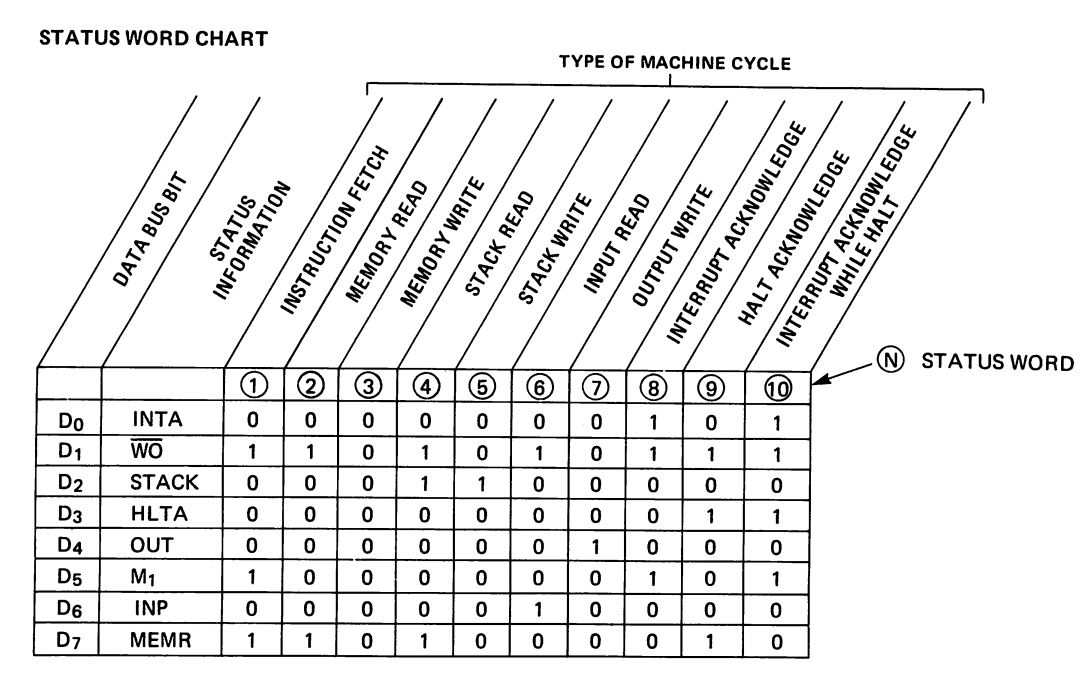
\includegraphics[width=15cm]{Bilder/Intel8080_DataLines}
\caption{Kodierung der Befehlstypen beim SYNC Takt \cite{IntMan20}}
\label{fig:status_word}
\end{figure}

\noindent
\textbf{Zustände, die zwei Takte dauern}

\noindent
Manche Zustände des Intel 8080 dauern zwei Takte an. Zu sehen ist das in Anhang \ref{anhang:instr_state}. Die Judge Condition, bei z.B. den bedingten Sprüngen, benötigt den vierten und fünften Zustand. Dies ist in diesem Simulator bisher nicht möglich. Deshalb 
wird der vierte Zustand ein leerer Zustand und der fünfte ist der eigentliche Zustand. 
\\

\noindent
Ähnliches ist auch bei anderen Zuständen der Fall. Ebenfalls bei den bedingte Sprüngen gibt es im zweiten Maschinenzyklus einen Zustand, der das zweite Byte in das Z-Register schreiben soll. Dies wurde aber so eingezeichnet, dass der Text \glqq B2\grqq\ noch im 2 Zustand und der Text \glqq Z\grqq\ im dritten Zustand steht. Deshalb wurde das Schreiben des zweiten Bytes in das Z-Register im dritten Zustand ausgeführt. Hier wurde der vorherige Zustand aber kein leerer Zustand, da dort der Programmzähler um eins erhöht werden muss.
\\

\noindent
\textbf{Abänderungen zum Handbuch}

\noindent
Bei den beiden MVI-Befehlen soll im zweiten Maschinenzyklus ein weiteres Byte gelesen werden. Bei allen anderen Befehlen, die ein zweites Byte lesen wird im zweiten Zustand des zweiten Zyklus der Programmzähler um eins erhöht. Dies ist deswegen notwendig, da sonst das gleiche Byte nochmal gelesen wird, was in der Zustandsbeschreibung allerdings fehlt. Damit der MVI-Befehl aber korrekt ausgeführt werden kann, wird auch dort der Programmzähler erhöht. Ebenso wurde beim DCR r-Befehl, der einen Wert um eins reduziert soll, der Wert um eins erhöht. Dies wurde im Simulator angepasst.
\\

\noindent
\textbf{Letzter Maschinenzyklus bei Sprungbefehlen}

\noindent
Bei allen Sprungbefehlen, die der Intel 8080 unterstützt, wird zuletzt ein WZ OUT STATUS-Signal gesendet und der Programmzähler auf den um eins erhöhten Wert des zusammengesetzten W- und Z-Registers gesetzt. Diese zwei Zustände werden in einem realen Prozessor anstatt des normalen Fetches des neuen Befehls ausgeführt. Dies ist in diesem Simulator aber nicht so einfach möglich. Deswegen haben alle Sprungbefehle einen zusätzlichen Maschinenzyklus erhalten. Dort wird nur der Wert des 16-Bit WZ-Registers in den Programmzähler geschrieben. Während des Fetch des nächsten Befehls wird dann der Zähler um eins erhöht. Somit führt das Programm an der richtigen Stelle weitere Befehle aus.
\\

\noindent
\textbf{Kleine Eigenheiten oder Unterschiede zum Prozessor}

\noindent
\begin{itemize}
\item Es wird überall nur mit unsigned Werten gearbeitet. Zero-Flag zeigt Werte > 127 (negative Werte) an
\item In der Beschreibung der Zustände werden teilweise Werte in die ALU geschrieben oder daraus gelesen (siehe Anhang \ref{anhang:instr_state} bei INR Befehl). Dies wird im Simulator nicht gemacht, da die arithmetischen Befehle nicht mehr in der ALU ausgeführt werden. Damit die Anzahl der Zustände wieder übereinstimmen, wurde der vierte Zustand in zwei aufgeteilt.
\item Es gibt keinen Hold-Modus, da die Busse nicht vom Prozessor freigegeben werden müssen.
\end{itemize}

\subsection{Laden und Anpassen der Oberfläche}\label{chapter:LadenDObfl}
Von Nico\\

\noindent
Die Oberfläche für den Simulator wurde nicht dynamisch erzeugt. Das heißt es existiert eine statische \glqq ui\grqq- Datei für jede Oberfläche mit der der Nutzer interagieren kann. Insgesamt gibt es die folgenden drei:\imgSpaceBefore

\begin{itemize}
	\item MainMenu.ui (Hauptmenü)
	\item Intel8080\_MainWindow.ui (Simulator)
	\item ChangeValueWindow.ui (Werte-Input)
\end{itemize}

\noindent
Als Beispiel für eins dieser manuell erstellten Fenster ist in Abbildung \ref{fig:RawUI} das Simulator-Fenster zu sehen.\imgSpaceBefore

\begin{figure}[H]
\centering
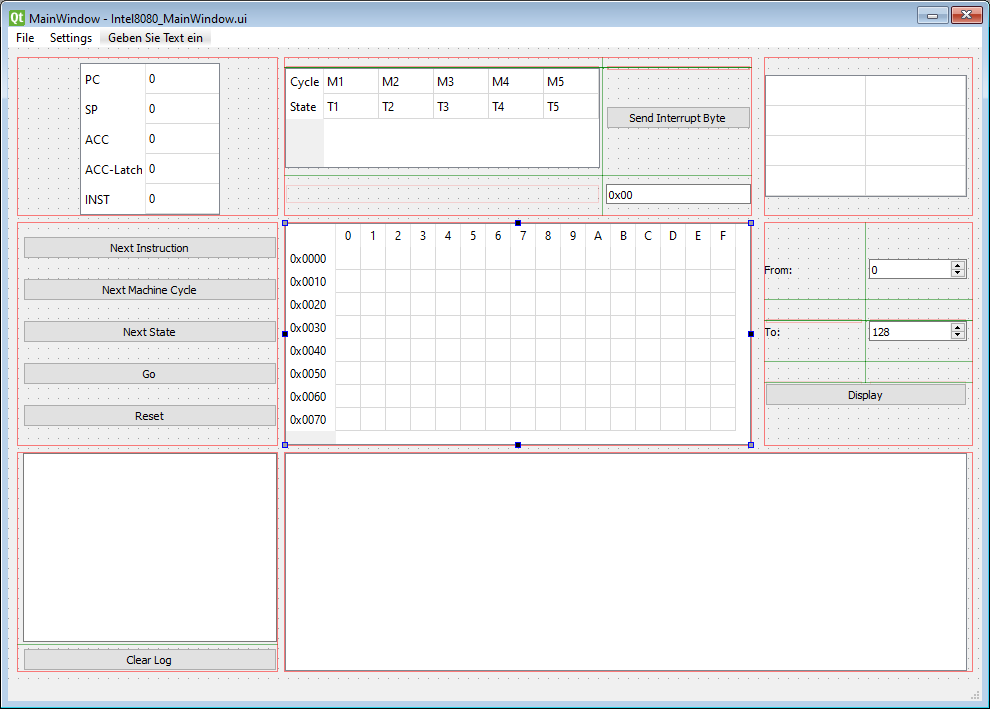
\includegraphics[width=15cm]{bilder/RawUIFile}
\caption{Rohes Simulator-Fenster}
\label{fig:RawUI}
\end{figure}

\noindent
In diesem wird jedem Element ein Name zugewiesen, über den dann später darauf zugegriffen werden kann. Über Layouts kann außerdem die grobe Position eines einzelnen Elements oder einer Gruppe von Elementen bestimmt werden. Vorteil dabei ist, dass unveränderliche Eigenschaften wie Elementtyp (Tabelle, Textfeld, etc.), bestimmte Beschriftungen oder Elementanzahlen (Spalten, Reihen, etc.) bereits festgelegt werden können, bevor die Implementierung der Funktionalität vorgenommen werden muss. Dadurch ist es einerseits möglich, eine Änderung schnell visuell zu überprüfen, und andererseits wird an komplizierter Syntax für Fenster gespart, was den Programmcode übersichtlicher hält. Verglichen mit der letztlich dem Nutzer angezeigten Oberfläche (siehe Abbildung \ref{fig:I8080MW}) fällt auf, dass die Größe einiger Elemente angepasst wurde und einige Knöpfe in die Zellen der Register-Elemente eingefügt wurden. Diese Anpassungen finden während der Initialisierung der \glqq Intel8080\_MainWindow\grqq-Klasse statt (siehe Abbildung \ref{fig:InitFuncs}).\imgSpaceBefore

\begin{figure}[H]
\centering
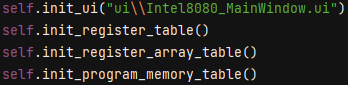
\includegraphics[width=8cm]{bilder/initFuncs}
\caption{Init-Functioncalls in Instanzfunktion für Intel 8080 Fenster}
\label{fig:InitFuncs}
\end{figure}

\vspace{15pt}

\begin{figure}[H]
\centering
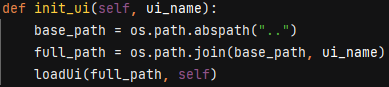
\includegraphics[width=8cm]{bilder/initUI}
\caption{Generische Funktion zum Laden der \glqq ui\grqq-Datei}
\label{fig:InitUI}
\end{figure}


\noindent
\glqq init\_ui\grqq ist hierbei eine generische Funktion die von allen Fenstern verwendet wird (siehe Abbildung  \ref{fig:InitUI}).
Aufgabe dieser ist es, den korrekten Pfad für die \glqq ui\grqq-Datei zu bestimmen und über den Funktionsaufruf \glqq loadUI\grqq die Datei in ein leeres QMainWindow zu laden. Die Funktionen für die Initialisierung der verschiedenen Register sowie des Programmspeichers erfüllen effektiv die gleiche Aufgabe. Das Bearbeiten der Werte wird über Knöpfe geregelt. Diese werden über die Initalisierungsfunktionen erzeugt und in die einzelnen Zellen des Elements eingefügt. Weiterhin wird den Knöpfen die Funktion \glqq pressed\_table\_cell\grqq zugewiesen, welche ausgeführt wird, sollte auf diese geklickt werden (um den Wert zu ändern). Ein Beispiel für eine der Funktionen, die diese Zuweisungen übernimmt, sieht man in Abbildung \ref{fig:InitProgMem}.\imgSpaceBefore

\begin{figure}[H]
\centering
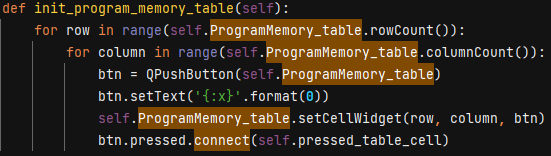
\includegraphics[width=12cm]{bilder/initProgMem}
\caption{Initialisierung des Programmspeichers}
\label{fig:InitProgMem}
\end{figure}

\noindent
Effektiv wird die in der \glqq ui\grqq-Datei definierte Anzahl Zeilen und Spalten der Programmtabelle abgefragt. Dann wird über jedes Element iteriert und ein Knopf erstellt mit Standardtext und einer Zuweisung. Die zugewiesene Funktion wird in Kapitel \ref{chapter:GUI-Methods} noch näher erklärt.


\subsection{GUI-Methoden}\label{chapter:GUI-Methods}
Von Nico\\

\noindent
Die GUI dient als Schnittstelle zwischen Benutzter und Prozessorsimulation. Die in diesem Abschnitt erklärten Funktionen beziehen sich deshalb auf die in Kapitel \ref{chp:AufbauGUI} beschriebenen Funktionen für die Benutzeroberfläche.

\subsubsection{Aktualisieren der Oberfläche}
Nach der Ausführung jedes Zustandes besteht die Möglichkeit, dass sich ein in der Oberfläche angezeigter Wert ändert, beispielsweise der Programmzähler im zweiten Zustand jedes Befehls. Um die Oberfläche regelmäßig zu aktualisieren, wurden folgende Funktionen verwendet:\imgSpaceBefore

\begin{itemize}
	\item reload\_registers\_table: Aktualisiert die besonderen Register wie Programmzähler, Instruction Register, etc.
	\item reload\_register\_array\_table: Aktualisiert generische 8-Bit Register (b, c, d, e, etc.)
	\item reload\_memory\_table: Aktualisiert Programmspeicher
	\item fill\_program\_table: Aktualisiert Programmtabelle
	\item color\_program\_table: Färbt die derzeit ausgeführte Zeile der Programmtabelle
	\item color\_cycle\_state: Färbt aktuellen Maschinenzyklus und Zustand in CycleState-Tabelle
\end{itemize}
\noindent
In der aktuellen Implementierung sind alle Funktionen jeweils so umgesetzt, dass alle relevanten Werte neu geladen werden, unabhängig davon, ob sie sich verändert haben oder nicht. Bei wenigen Werten, z.B. für die Register, stellt dies noch kein Problem dar, aber für den Programmspeicher (jeweils 128 8-Bit Register werden auf einmal ausgelesen) und vor allem für die Programmtabelle (komplettes Parsen und Filtern des Programmspeichers sowie Füllen der Tabelle) macht sich dies erheblich in der Performance bemerkbar. Da bisher noch kein Verfahren implementiert wurde, mit dem bei Bedarf selektiv aktualisiert werden kann, müssen bei jeder Zustandsänderung alle Funktionen für die Aktualisierung der Oberfläche ausgeführt werden. Dies geschieht über die \glqq update\_ui\grqq-Funktion (siehe Abbildung \ref{fig:updateUI}).\imgSpaceBefore

\begin{figure}[H]
\centering
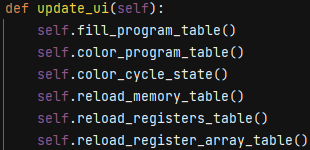
\includegraphics[width=8cm]{bilder/updateUI}
\caption{update\_ui Funktion}
\label{fig:updateUI}
\end{figure}

\noindent
Die \glqq update\_ui\grqq-Funktion wird innerhalb der Klasse für die Simulatoroberfläche an mehreren Stellen verwendet:\imgSpaceBefore

\begin{itemize}
	\item Zu Beginn bei Initialisierung der Oberfläche
	\item Bei Laden eines neuen Programms über die Benutzeroberfläche
	\item Bei Zurücksetzen des Simulators über den Reset-Knopf
	\item Bei automatischen Ausführen des Programms über den Go-Knopf (Aktualisieren nach jeder Instruction)
	\item Nach Ausführen einer Instruction, eines Machinenzyklus oder eines Zustandes über die jeweiligen Knöpfe
\end{itemize}

\noindent
Wie bereits erwähnt, ist der Sinn dieser Maßnahme, dass keine Veränderung der angezeigten Aspekte des Simulators übersehen wird. Schlimmstenfalls könnte es auch dazu führen, dass wenn eine Anzeige nicht aktualisiert wird, dieser fehlerhafte Wert nach Manipulieren eines anderen fälschlicherweise in die internen Register des Simulators zurückgeschrieben wird. Dieses Prinzip sieht man in Abbildung \ref{fig:perf}.\imgSpaceBefore

\begin{figure}[H]
\centering
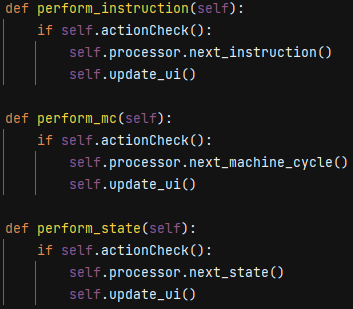
\includegraphics[width=8cm]{bilder/Perform}
\caption{Programmschritte Instruction/Cycle/State}
\label{fig:perf}
\end{figure}

\noindent
Die Implementierungen der drei Knöpfe zum Ausführen eines Befehl, eines Maschinenzyklus oder eines Zustandes sind lediglich Anweisungen an den Simulator, diese abzuarbeiten, woraufhin über \glqq update\_ui\grqq die gesammelten Informationen wieder in die Benutzeroberfläche geladen werden. Ähnlich wie die \glqq update\_ui\grqq-Funktion alle Elemente aktualisiert arbeiten auch die einzelnen Funktionen darin. Als Beispiel dafür ist in Abbildung \ref{fig:reloadRegs} die Funktion zum aktualisieren der Oberfläche für die speziellen Register zu sehen.\imgSpaceBefore

\begin{figure}[H]
\centering
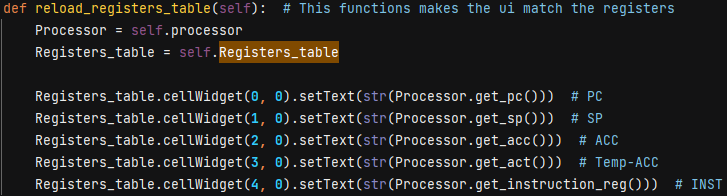
\includegraphics[width=14cm]{bilder/reloadRegs}
\caption{Special Register Refresh}
\label{fig:reloadRegs}
\end{figure}

\noindent
Da es schwer nachzuvollziehen ist wann ein Bestandteil eines Elements des Simulators seinen Zustand ändert (beispielsweise ein einzelnes Register im Speicher), liest die Funktion einfach über die im Simulator definierte Schnittstellen alle für das Element relevanten Werte aus und trägt sie im korrekten Format in die Tabelle ein. Dieses Verhalten gilt auch in ähnlicher Weise für die \glqq reload\_register\_array\_table\grqq- und die \glqq reload\_program\_memory\_table\grqq-Funktion. Etwas anders funktioniert die Funktion, welche den Programmspeicher parst (\glqq fill\_program\_table\grqq) um das Programm übersichtlich mit der entsprechenden Bedeutung des Bytebefehls darzustellen (siehe Abbildung \ref{fig:FillProgReg}).\imgSpaceBefore

\begin{figure}[H]
\centering
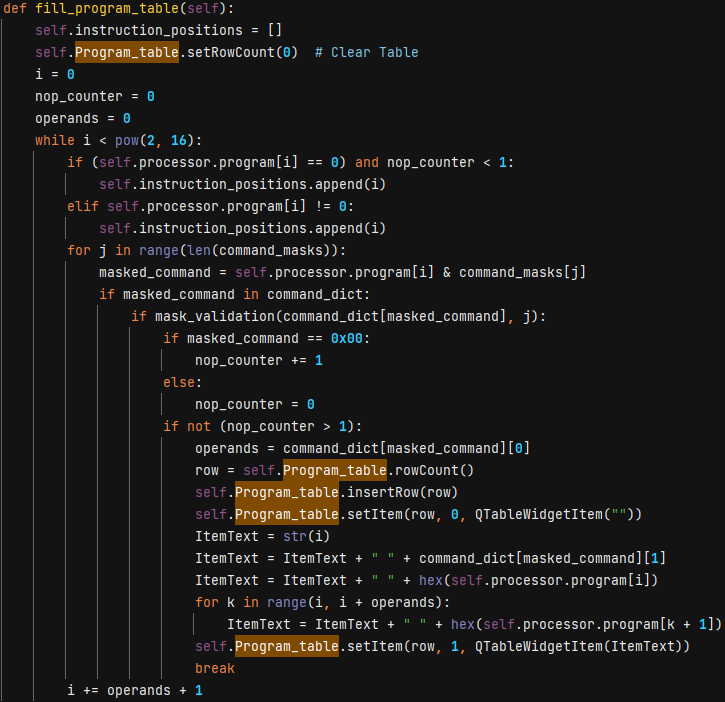
\includegraphics[width=14cm]{bilder/FillProgTable}
\caption{Program Table Function}
\label{fig:FillProgReg}
\end{figure}

\noindent
Zuerst werden alle Einträge der Tabelle gelöscht woraufhin über alle Register im Programmspeicher iteriert wird. Da in jedem Eintrag der Tabelle ein Befehl, sowie dessen Operanden stehen sollen, wird über eine Liste (instruction\_positions) der Index jedes Befehls gespeichert. Dadurch soll sichergestellt werden, dass Operanden in die selbe Zeile geschrieben werden wie der Befehl zu dem sie gehören. Das bestimmen des Befehls sowie der Anzahl Operanden pro Befehl geschieht über ein Dictionary. Die Abfrage funktioniert so funktioniert so, dass die Masken für jeden Befehl mit dem Bytecode im Programmspeicher verundet werden und geschaut wird ob sich der resultierende Eintrag im Dictionary findet (siehe Abbildung \ref{fig:Dict}).\imgSpaceBefore

\begin{figure}[H]
\centering
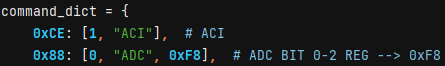
\includegraphics[width=12cm]{bilder/CmdDictExample}
\caption{Dictionary Ausschnitt}
\label{fig:Dict}
\end{figure}

\noindent
Die Einträge sind hierbei die Anzahl der nachfolgenden Operanden, die Bezeichnung des Befehls und, falls angewendet, die Maske zum bestimmen des Befehls. Um keine zufälligen Treffer zu erzielen (beispielsweise verunden mit falscher Maske führt zu anderem Befehl) wird nach einer Übereinstimmung im Dictionary die \glqq mask\_validation\grqq-Funktion verwendet (siehe Abbildung \ref{fig:MaskValid}).\imgSpaceBefore

\begin{figure}[H]
\centering
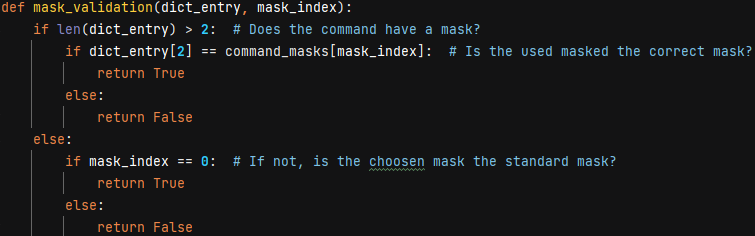
\includegraphics[width=14cm]{bilder/mask_valid}
\caption{Mask Validation Function}
\label{fig:MaskValid}
\end{figure}

\noindent
Hierbei wird zuerst überprüft ob der vermeintliche Befehl eine Maske verwendet und dann ob die angewendete Maske die korrekte Maske ist. Falls der Befehl keine Maske verwendet wird geprüft ob auch keine verwendet wurde. Ist das Ergebnis negativ wird die Übereinstimmung verworfen. Bei einem gültigen Treffer wird ein Eintrag in der Tabelle angelegt der die Stelle im Speicher, den Namen des Befehls sowie dessen Operanden umfasst. Dabei wird berücksichtigt ob es sich um einen NOP-Befehl handelt. Da leere Speicherstellen als dieser interpretiert werden, wurde sich dazu entschieden diese Einträge zusammenzufassen insofern mehrere aufeinanderfolgen. Dies wird mit einem einfachen Zähler erreicht. Am Ende der Schleife werden die Anzahl Operanden auf die Zählvariable \glqq i\grqq addiert um die Einträge der Operanden zu überspringen.

\subsubsection{Manipulieren der Simulation}
Das zurückschreiben von der GUI in den Simulator geschieht über drei verschiedene Funktionen:\imgSpaceBefore

\begin{itemize}
	\item update\_registers\_table (PC, Instr, ACC, etc.)
	\item update\_register\_array\_table (b, c, d, e, etc.)
	\item update\_memory\_table (Programmspeicher)
\end{itemize}

\noindent
Diese funktionieren ähnlich wie deren Initalisierungsfunktionen (siehe Kapitel \ref{chapter:LadenDObfl}). Dabei wird über jede gültige Zelle der Tabelle iteriert, der Wert herausgeschrieben und über eine gültige Funktion in den Intel8080-Simulator übernommen. Als Beispiel dafür ist in Abbildung \ref{fig:MemUpdateFunc} die konkrete Implementierung für das Zurückschreiben des Programmspeichers zu sehen.\imgSpaceBefore

\begin{figure}[H]
\centering
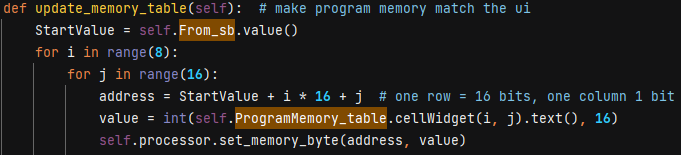
\includegraphics[width=15cm]{bilder/UpdateProgMem}
\caption{Memory Update-Function}
\label{fig:MemUpdateFunc}
\end{figure}

\noindent
Zuerst wird bestimmt welcher Speicherbereich derzeit angezeigt wird. Da die Programmspeichertabelle immer genau acht Zeilen und sechzehn Spalten hat (also 128 Register) können diese Werte fix verwendet werden. Daraufhin wird für jede Zeile die Adresse berechnet. Der Wert wird aus den Knöpfen bezogen und zur Basis 10 umgerechnet, da diese in Hexadezimal-Darstellung als String in diesen gespeichert werden. Über die Prozessorfunktion \glqq set\_memory\_byte\grqq werden die Werte dann einzeln zurückgeschrieben. Die drei \glqq update\grqq-Funktionen werden im Gegensatz zu den \glqq reload\grqq-Funktionen nur aufgerufen wenn tatsächlich ein Wert im jeweiligen Element ändert. Dabei ist die bereits angesprochene Funktion welche mit den Knopfelementen dieser Tabellen verknüpft ist relevant (siehe \ref{fig:PTC}).\imgSpaceBefore

\begin{figure}[H]
\centering
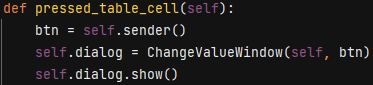
\includegraphics[width=12cm]{bilder/PTC}
\caption{Knopfdruck Funktion}
\label{fig:PTC}
\end{figure}

\noindent
Dabei wird der Knopf welcher die Funktion aufruft als Referenz an das neu erzeugte ChangeValueWindow übergeben. Dieser wird benötigt um zu bestimmen welches Element eine Werteänderung vornimmt. In Abbildung \ref{fig:CheckInput} ist die Funktion des ChangeValueWindow zu sehen welche die Eingabevalidierung vornimmt und die für das Element entsprechende \glqq update\grqq-Funktion aufruft.\imgSpaceBefore

\begin{figure}[H]
\centering
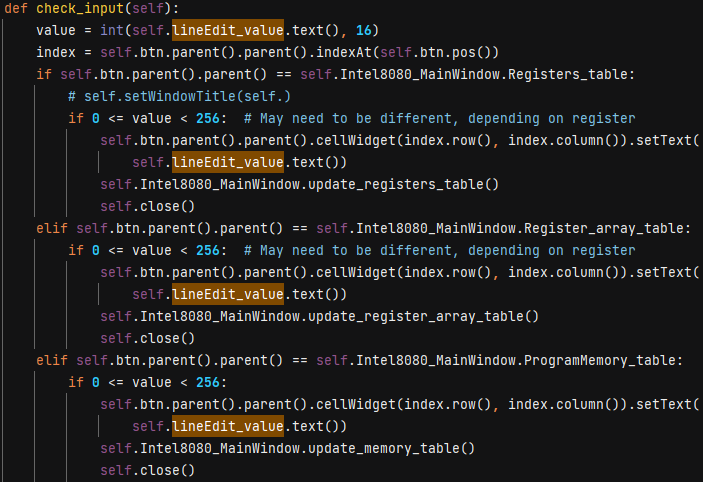
\includegraphics[width=12cm]{bilder/CheckInput}
\caption{InputValidation Function}
\label{fig:CheckInput}
\end{figure}

\noindent
Als erstes wird der Wert ausgelesen und der Index des Knopfes innerhalb der Tabelle bestimmt. Danach wird geprüft aus welchem Element der aufrufende Knopf stammt.

\subsubsection{Sonstige Interaktionen}
Da das gesamte Auslesen und Anzeigen der 65.536 8-Bit Register zu lange dauern würde und eher unnötig ist, wurde die Anzeige der Programmspeichertabelle auf 128 aufeinanderfolgende Register limitiert. Um auswählen zu können welche Register angezeigt werden, sind zwei Eingabefenster vorgesehen. Entweder um anzugeben bis zu oder ab welchem Register der Speicher angezeigt werden soll. Das Ändern des einen Wertes passt dabei den anderen automatisch an.\imgSpaceBefore

\begin{figure}[H]
\centering
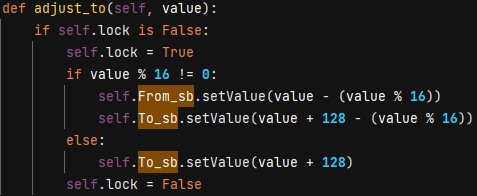
\includegraphics[width=12cm]{bilder/Range_to}
\caption{Range Funktion}
\label{fig:RangeTo}
\end{figure}

\noindent
Dafür wird ein Signal, welches ausgelöst wird sobald sich der Wert ändert mit der in Abbildung \ref{fig:RangeTo} gezeigten Funktion verknüpft. Um zu verhindern, dass die beiden Funktionen sich in einer Endlosschleife gegenseitig aufrufen wird ein Lock verwendet. Die Oberfläche wird nicht sofort aktualisiert, dafür muss zuerst der darunterliegende Knopf gedrückt werden, oder der Zustand des Simulators verändert werden.

\newpage
\subsubsection{Exe-Erstellung}
Als letzter Schritt wurde für das Programm noch eine .exe-Datei erstellt. Um zwischen den Versionen zu unterscheiden, wurde zu jeder Exe-Datei der entsprechende Commit angegeben. Aufgrund von Schwierigkeiten den Pfad der Dateien welche die Benutzeroberfläche definieren für die Exe-Dateien korrekt festzulegen bzw. diese direkt in das Program zu integrieren, müssen diese auf eine spezielle Art aufgerufen werden. Die Exe-Datei muss aus dem Basispfad des Programms heraus ausgeführt werden. Dabei wird lediglich das Verzeichnis unter 8-Bit-Simulator\textbackslash Code\textbackslash ui sowie deren Inhalt benötigt, der Pfad muss aber identisch sein (siehe Beispiel \ref{fig:OrdnerStruk}).\imgSpaceBefore

\begin{figure}[h]
\centering
\begin{subfigure}{.25\textwidth}
  \centering
  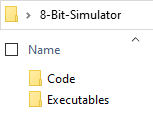
\includegraphics[width=.7\linewidth]{bilder/o1}
\end{subfigure}%
\begin{subfigure}{.35\textwidth}
  \centering
  \includegraphics[width=.7\linewidth]{bilder/o2}
\end{subfigure}
\begin{subfigure}{.35\textwidth}
  \centering
  \includegraphics[width=.7\linewidth]{bilder/o3}
\end{subfigure}
\caption{Ordnerstruktur}
\label{fig:OrdnerStruk}
\end{figure}

\noindent
Während dies recht umständlich ist, bietet es zumindest den Vorteil, dass keine Python-Umgebung sowie die benötigten Pakete auf dem Rechner installiert werden müssen. Sollte keine aktuelle Version des Programms als ausführbare Datei vorliegen wird eine Python Installation (Version 3.9 oder 3.10 getestet und funktionieren) und das PyQt6 Paket \cite{qt} benötigt.

\section{Fazit und Ausblick}
Von Nico \\

\noindent
\subsection{Zusammenfassung}
Das Ergebnis dieser Studienarbeit ist ein Simulator für den Intel 8080 welcher mit einer zugehörigen Benutzeroberfläche bedient werden kann. Die relevanten Aspekte des Prozessors werden dem Nutzer dabei angezeigt, wie beispielsweise Registerinhalte, das ausgeführte Programm oder einzelne Operationen für jeden Zustand. Es ist dem Nutzer möglich eigene Programme über die Benutzeroberfläche in den Simulator einzufügen oder diese zuvor über den verwendeten Assembler zu erstellen und dann direkt einzulesen. Die eingefügten Programme können Schrittweise ausgeführt werden, wobei es möglich ist ganze Befehle, Maschinenzyklen oder sogar einzelne Zustände auszuführen. Die Bedeutung einzelner Zustände wird in einem Befehlslog eingetragen um nachvollziehen zu können was in jedem Zustand passiert. Programme können automatisch ausgeführt werden und über Haltepunkte auch automatisch an einer beliebigen Stelle angehalten werden. Es ist zu jedem Zeitpunkt möglich die internen Aspekte des Simulators zu verändern über eine einfach zu bedienende Oberfläche. Das zurücksetzen der Oberfläche funktioniert auch problemlos. Der gesamte Befehlssatz des Intel 8080 wurde so genau wie möglich implementiert und sollte identische Ergebnisse liefern wie nativ ausgeführte Operationen.

\subsection{Ausblick}
Die Benutzeroberfläche ist derzeit vollständig in Englisch geschrieben. Es wäre also eine Überlegung Wert eine Einstellung einzufügen für andere Sprachen. Der Befehlslog ist aktuell noch recht kryptisch. Während es wenn man die Bedeutung der Zustände und Abkürzung kennt zwar genügend Aufschluss gibt, ist diese Variante noch verbesserungswürdig. Das Erstellen eigener Programme ist nur über die Programmspeichertabelle möglich, bisher wurde kein eigener Editor entwickelt. Externes Erstellen muss über den mitgelieferten Assembler vorgenommen werden, wobei dafür keine eigene Bedienungsanleitung verfasst wurde. Eine interne Lösung auch mit Hilfestellung für die einzelnen Bytebefehle und deren Bedeutung wäre erstrebenswert. Das Tutorial vermittelt die notwendigen Grundlagen um den Simulator zu bedienen, aber eine interaktive Lösung mit Beispielen hätte vermutlich einen höheren Lernerfolg.

\newpage


\addcontentsline{toc}{section}{Literatur}
\begin{thebibliography}{9}

\bibitem{Adressformate}Instruction formats: \url{https://www.geeksforgeeks.org/computer-organization-instruction-formats-zero-one-two-three-address-instruction/}, zuletzt abgerufen: 25.12.2021

\bibitem{Architektur_stud}
Von-Neumann vs. Harvard: Studyflix,	\url{https://studyflix.de/informatik/von-neumann-vs-harvard-786}, zuletzt abgerufen: 15.05.2022

\bibitem{Architektur}
Von Neumann Architektur: \url{https://de.wikipedia.org/wiki/Von-Neumann-Architektur}, zuletzt abgerufen: 15.05.2022

\bibitem{Herold}
Grundlagen der Informatik: Herold, Lurz, Wohlrab und Hopf; 3. aktualisierte Auflage (2017), Pearson

\bibitem{Flynn}
Some Computer Organizations and Their Effectiveness (S.948-960, vol. C-21): M. J. Flynn, 1972, in IEEE Transactions on Computers

\bibitem{IntMan16}
Intel 8080 Microcomputer Systems User's Manual (S.16 (2-2)): Intel Corporation, 1975, \url{http://bitsavers.trailing-edge.com/components/intel/MCS80/98-153B_Intel_8080_Microcomputer_Systems_Users_Manual_197509.pdf} zuletzt abgerufen: 14.05.2022

\bibitem{IntMan30}
Intel 8080 Microcomputer Systems User's Manual (S.30 ff. (2-16)): Intel Corporation, 1975, \url{http://bitsavers.trailing-edge.com/components/intel/MCS80/98-153B_Intel_8080_Microcomputer_Systems_Users_Manual_197509.pdf} zuletzt abgerufen: 14.05.2022

\bibitem{IntMan45}
Intel 8080 Microcomputer Systems User's Manual (S.46 ff. (4-1)): Intel Corporation, 1975, \url{http://bitsavers.trailing-edge.com/components/intel/MCS80/98-153B_Intel_8080_Microcomputer_Systems_Users_Manual_197509.pdf} zuletzt abgerufen: 14.05.2022

\bibitem{IntMan18}
Intel 8080 Microcomputer Systems User's Manual (S.18 f. (2-4)): Intel Corporation, 1975, \url{http://bitsavers.trailing-edge.com/components/intel/MCS80/98-153B_Intel_8080_Microcomputer_Systems_Users_Manual_197509.pdf} zuletzt abgerufen: 14.05.2022

\bibitem{Assembler}
Intel 8080 Assembler: Paolo Amoroso, 2021, \url{https://github.com/pamoroso/suite8080/tree/56c2e077dd3d178859d614932b9a1f33fa238e21}, zuletzt abgerufen: 15.05.2022

\bibitem{IntMan20}
Intel 8080 Microcomputer Systems User's Manual (S.20 (2-6)): Intel Corporation, 1975, \url{http://bitsavers.trailing-edge.com/components/intel/MCS80/98-153B_Intel_8080_Microcomputer_Systems_Users_Manual_197509.pdf} zuletzt abgerufen: 14.05.2022

\bibitem{qt}
PyQt Reference Guide, \url{https://www.riverbankcomputing.com/static/Docs/PyQt6/index.html}, zuletzt abgerufen: 15.05.2022

\end{thebibliography}

\newpage
\thispagestyle{empty}


\appendix
\section*{Anhang}
\addcontentsline{toc}{section}{Anhang}

\applabel{anhang:instr_state}
\includepdf[pages={30-33}]{../Datenblaetter/Intel 8080.pdf}



\end{document}
